\documentclass[a4paper,10pt]{article}

% ------------------------------------
% packages
\usepackage[a4paper,margin=1in,footnotesep=2.2\baselineskip]{geometry}
\usepackage{multicol}
\usepackage{xcolor}
\usepackage{framed}
\usepackage{emoji}
\usepackage[most]{tcolorbox}
\usepackage{fancyhdr}
\usepackage[tracking=true]{microtype}
\usepackage{ragged2e}
\usepackage{listings}
\usepackage{color}
\usepackage{pagecolor}
\usepackage{pdftexcmds}
\usepackage{geometry}
\usepackage{upgreek}
\usepackage{accents}
\usepackage{caption}
\usepackage{amssymb}
\captionsetup{
  font=small,
  labelfont=bf,
  tableposition=top
}
\captionsetup[figure]{name=\mono{Figure}}

% ------------------------------------
% checksum = SHA-1
\makeatletter
\ifx\pdf@filemdfivesum\undefined\def\pdf@filemdfivesum#{\mdfivesum file}\fi
\let\filesum\pdf@filemdfivesum
\makeatother

% ------------------------------------
% color definitions
\definecolor{armygreen}{rgb}{0.14, 0.71, 0.15}
\definecolor{darkgreen}{rgb}{0.08, 0.48, 0.18}
\definecolor{darkred}{rgb}{0.86, 0.153, 0.153}
\definecolor{azure}{rgb}{0.0, 0.5, 1.0}
\definecolor{bole}{rgb}{0.82, 0.57, 0.22}
\definecolor{dkgreen}{rgb}{0,0.6,0}
\definecolor{gray}{rgb}{0.5,0.5,0.5}
\definecolor{mauve}{rgb}{0.58,0,0.82}
\definecolor{light-gray}{gray}{0.95}
\definecolor{bg}{HTML}{fcfcfa}
\definecolor{bt}{HTML}{ffebe6}

% ------------------------------------
% code styling
\definecolor{shadecolor}{RGB}{180,180,180}
\newcommand{\code}[1]{\colorbox{shadecolor!30}{\mono{#1}}}
\newcommand{\zero}{{\raisebox{-0.7ex}{\LARGE\starg{o}}}}

% ------------------------------------
% digits
%\newcommand{\one}{{$\aleph$}}
%\newcommand{\two}{3}
%\newcommand{\three}{\uptheta}
%\newcommand{\four}{k}
%\newcommand{\five}{\raisebox{0.55ex}{\naskh{^^^^062d}}}
%\newcommand{\six}{{\hindi{^^^^096d}}}
%\newcommand{\seven}{\raisebox{0.3ex}{\robot{^^^^0434}}}
\newcommand{\one}{{\raisebox{-0.7ex}{\LARGE\starg{y}}}}
\newcommand{\two}{{\raisebox{-0.7ex}{\LARGE\starg{s}}}}
\newcommand{\three}{{\raisebox{-0.7ex}{\LARGE\starg{e}}}}
\newcommand{\four}{{\raisebox{-0.7ex}{\LARGE\starg{w}}}}
\newcommand{\five}{{\raisebox{-0.7ex}{\LARGE\starg{g}}}}
\newcommand{\six}{{\raisebox{-0.7ex}{\LARGE\starg{x}}}}
\newcommand{\seven}{{\raisebox{-0.7ex}{\LARGE\starg{t}}}}
\newcommand{\asserts}{\raisebox{0.10ex}{$\equiv$}}
\colorlet{Gray}{gray!20!}
\tcbset{on line, arc=1pt, leftrule=0.25pt,rightrule=0.25pt,toprule=0.25pt,bottomrule=0.25pt,
  boxsep=3pt, left=0pt,right=0pt,top=0pt,bottom=0pt,
  colframe=white,colback=Gray,  
  highlight math style={enhanced}
}
\lstdefinelanguage{Solidity}{
  %keywords={bool, true, false, return, address, bytes32, bytes4, bytes1, bytes, uint256, uint8, uint, string, if, while, else, case, break},
  keywords={},
  keywordstyle=\color{blue}\bfseries,
  %ndkeywords={function,struct, mapping, export, throw, implements, import, this},
  ndkeywords={},
  ndkeywordstyle=\color{darkgreen}\bfseries,
  identifierstyle=\color{black},
  sensitive=false,
  comment=[l]{//},
  morecomment=[s]{/*}{*/},
  commentstyle=\color{green}\mono,
  stringstyle=\color{orange}\mono,
  morestring=[b]',
  morestring=[b]",
  mathescape=true,
  literate={=>}{${\rightarrow}{}$}{1}
}
\lstset{
  backgroundcolor=\color{light-gray},
  language=Solidity,
  aboveskip=3mm,
  belowskip=3mm,
  showstringspaces=false,
  columns=flexible,
  basicstyle={\footnotesize\mono},
  numbers=none,
  numberstyle=\tiny\color{gray},
  keywordstyle=\color{blue},
  commentstyle=\color{dkgreen},
  stringstyle=\color{mauve},
  breaklines=true,
  breakatwhitespace=true,
  tabsize=3
}

% ------------------------------------
% fonts
\newfontfamily\pro[Path=./]{SFPro.ttf}
\newfontfamily\pbold[Path=./]{SFMonoSemiBold.ttf}
\newfontfamily\mono[Path=./]{SFMono.ttf}
\newfontfamily\mbold[Path=./]{SFMonoSemiBold.ttf}
\newfontfamily\hindi[Path=./]{Martel.ttf}
\newfontfamily\kalam[Path=./]{Kalam.ttf}
\newfontfamily\naskh[Path=./]{Naskh.ttf}
\newfontfamily\robot[Path=./]{Roboto.ttf}
\newfontfamily\victr[Path=./]{VictorMono.ttf}
\newfontfamily\pala[Path=./]{Palatino.ttf}
\newfontfamily\mate[Path=./]{Mate.ttf}
\newfontfamily\starg[Path=./]{Stargate.ttf}

% ------------------------------------
% heading font-size
\usepackage{sectsty}
\usepackage{fontspec}
\sectionfont{\fontsize{12}{15}\selectfont}
\usepackage[utf8]{inputenc}

% ------------------------------------
% footnote positioning
\usepackage[hang,flushmargin,bottom]{footmisc} 

% ------------------------------------
% bibliography
\usepackage[colorlinks=true,
            linkcolor=blue,
            urlcolor=blue,
            citecolor=blue,
            pdfauthor={sshmatrix},
            pdftitle={Helix2 Protocol},
            pdfsubject={Link Service and Protocol},
            pdfkeywords={ethereum, account, abstraction, link, name, decentralised, distributed},
            pdfproducer={sshmatrix},
            pdfcreator={sshmatrix}]{hyperref}
            
% ------------------------------------
% blank footnote
\newcommand\blfootnote[1]{%
  \begingroup
  \renewcommand\thefootnote{}\footnote{#1}%
  \addtocounter{footnote}{-1}%
  \endgroup
}

% ------------------------------------
% header
\pagestyle{fancy}
\fancyhf{}
\lfoot{\footnotesize \mono{\#}\tcbox{\mono{\filesum{\jobname}}}}
\begin{document}
\setcounter{footnote}{0}
\newpage
\topskip15pt

\fancyhead[L]{\footnotesize \mono{author}:\tcbox{\mono{sshmatrix}}}
\fancyhead[R]{{\footnotesize \mono{\href{https://github.com/sshmatrix/research}{github.com/sshmatrix/research/ecTopology}}}}
\fancyhead[C]{{\footnotesize \emoji{dna}}}
\fancyfoot[C]{{\footnotesize \mono{\thepage}}}
\fancyfoot[R]{{\footnotesize \mono{\today} \emoji{dna}}}

\begin{center}
  \textbf{\Large\pbold{\textls[-40]{Topological Interpretation of Elliptic Curves}}}\\
  \vspace{0.075in}
  \textls[-50]{\mono{Topological Interpretation of Finite Cyclic Groups}}\linebreak\linebreak
  \vspace{-0.175in}
  \textls[0]{\mono{Avneet Singh}}\linebreak\linebreak
  \textls[0]{\mono{SysStruct}}\linebreak
  \textls[0]{\mono{\href{mailto:sshmatrix@pm.me}{sshmatrix@pm.me}}}\linebreak
\end{center}
\begin{center}
  \textbf{\Large\pbold{ABSTRACT}}\linebreak\linebreak
  \textls[-50]{\mono{Elliptic curves form the backbone of most cryptography today and are expected to feature in the post-quantum world through Zero-Knowlege algorithms. Most literature on Elliptic curves starts from the definition of a cubic symmetric polynomial and builds upon the group theoretic interpretation of finite fields. This may be sufficient to grasp the mere necessary details for implementing Elliptic curves in practise, but not necessarily ideal if one wants to understand why Elliptic curve geometry is unique and useful. To most readers, it can appear that Elliptic curves were drawn from a magic hat. In paper will illustrate that this is clearly not the case and there exists a very legitimate reason for how and why the humanity ended up using Elliptic curves for cryptography.}}
\end{center}
\vspace{0.2in}
\begin{flushleft}
  \textbf{\Large\pbold\textls[-25]{INTRODUCTION}}\linebreak\linebreak
  \textls[-50]{\mono{This paper is intended as a standalone appendix to the main paper titled 'Intuitive Interpretation of Non-Interactive Zero-Knowledge Cryptography' [1]. The main paper deals with pretty much the entire field of cryptography starting from basic RSA to advanced Zero-Knowledge algorithms. In interest of conciseness, several important aspects of Elliptic curves couldn't be discussed in detail in the main paper; this document is an attempt to address those shortcomings for the overtly inclined reader. We'll also touch some peripheral topics that have tied number theory and elliptic curves at the hip. Having said that, we'll follow the same theme as the main paper and avoid jargon like plague.\linebreak\linebreak\linebreak
  }}
  \textbf{\Large\pbold\textls[-25]{ARC-LENGTH OF AN ELLIPSE}}\linebreak\linebreak
  \textls[-50]{\mono{The hint is in the name. Elliptic curves are related to ellipses and their discovery was 'accidental' so to speak; most of the initial work toward elliptic curves was done by Newton, Legendre, Fermat, Euler, Abel and Jacobi. In simple terms, an elliptic curve is a paramterisation of an ellipse's circumference or arc length and it easily derivable. To begin with, consider an ellipse described by  its semi-major and -minor axis lengths of \resizebox{7.25px}{5.3px}{\upalpha} and \raisebox{0.25mm}{\resizebox{6.5px}{5px}{\upgamma}} (=\;1), i.e. eccentricity e\textsuperscript{2} = 1 - {1/\resizebox{7.25px}{5.3px}{\upalpha}}\textsuperscript{2}. Such an ellipse is described by: {{(1 - e\textsuperscript{2})}}\,{{x\textsuperscript{2}}} + {y\textsuperscript{2} = 1}. We can simplify it further by safely\textsuperscript{\textcolor{blue}{1}}\blfootnote{\textls[-50]{\mono{\textsuperscript{1}{such that the values of both e and k lie between 0 and 1, aka [0, 1]}}}} replacing the constant 1 - e\textsuperscript{2} with k\textsuperscript{2}, yielding $\text{y\textsuperscript{2} = 1 - {\text{k\textsuperscript{2}}}\,{\text{x\textsuperscript{2}}}}$. Let's try to calculate the circumference C(k) of this ellipse; this will be equivalent to integrating ({\resizebox{5px}{7px}{\updelta}}x\textsuperscript{2} + {\resizebox{5px}{7px}{\updelta}}y\textsuperscript{2})\textsuperscript{1/2} along the curve in one of the four cartesian quarters and then multiplying it by 4. This results in
  \vspace{2mm}
  \begin{center}
    C(e) = 4\;\raisebox{-1mm}{\huge\mate{^^^^222b}}({\resizebox{5px}{7px}{\updelta}}x\textsuperscript{2} + {\resizebox{5px}{7px}{\updelta}}y\textsuperscript{2})\textsuperscript{1/2}, for x = [0, \resizebox{7.25px}{5.3px}{\upalpha}],
  \end{center}
  \begin{flushright}
    {\vspace{-8mm}\mono{(1)}}
  \end{flushright}
  \vspace{2mm}
  \begin{center}
    C(e) = 4\;{{\raisebox{-1mm}{\huge\mate{^^^^222b}}}\textsuperscript{\raisebox{2.5mm}{\scriptsize{\upalpha}}}}{\hspace{-2.75mm}\textsubscript{\raisebox{-2.5mm}{\footnotesize{0}}}}\;({\resizebox{5px}{7px}{\updelta}}x\textsuperscript{2} + {\resizebox{5px}{7px}{\updelta}}y\textsuperscript{2})\textsuperscript{1/2} = 4\;{{\raisebox{-1mm}{\huge\mate{^^^^222b}}}\textsuperscript{\raisebox{2.5mm}{\scriptsize{\upalpha}}}}{\hspace{-2.75mm}\textsubscript{\raisebox{-2.5mm}{\footnotesize{0}}}}\;\Big[$\displaystyle\frac{\text{1 - e\textsuperscript{2}x\textsuperscript{2}}}{\text{1 - x\textsuperscript{2}}}$\Big]\textsuperscript{\textsuperscript{\scriptsize{1/2}}}\,{\resizebox{5px}{7px}{\updelta}}x.
  \end{center}
  \begin{flushright}
    {\vspace{-8mm}\mono{(2)}}
  \end{flushright}
  \vspace{1.85mm}
  This is already the {\mbold{elliptic integral}} of the second kind{\textsuperscript{\textcolor{blue}{2}}\blfootnote{\textls[-50]{\mono{\textsuperscript{2}{'second kind' due to the presence of {\uptheta} in the numerator in its parameterised form; 'first kind' has 1 in the numerator}}}}} and it is particularly difficult to evaluate analytically. When e = 1 (i.e. straight lines; k = 0), it is straightforward and evaluates to 4$\text{\resizebox{7.25px}{5.3px}{\upalpha}}$ as expected. When e = 0 (i.e. circles; k = 1), it is also relatively straightforward and evaluates naturally to
  \vspace{1mm}
  \begin{center}
    C(e)\textsubscript{k\,=\,1} = 4\;{{\raisebox{-1mm}{\huge\mate{^^^^222b}}}\textsuperscript{\raisebox{2.5mm}{\scriptsize{\upalpha}}}}{\hspace{-2.75mm}\textsubscript{\raisebox{-2.5mm}{\footnotesize{0}}}}\;$\displaystyle\frac{\text{1}}{\text{(1 - x\textsuperscript{2})\textsuperscript{1/2}}}$\,{\resizebox{5px}{7px}{\updelta}}x = 4\;{{\raisebox{-1mm}{\huge{$|$}}}\hspace{-0.2mm}\textsuperscript{\raisebox{2mm}{\scriptsize{\upalpha}}}}{\hspace{-2.15mm}\textsubscript{\raisebox{-2.5mm}{\footnotesize{0}}}}\;sin\textsuperscript{-1}(x) = 2\hspace{0.2mm}{\resizebox{5.25px}{5.25px}{\uppi}}\hspace{0.2mm}\resizebox{7.25px}{5.3px}{\upalpha}.
  \end{center}
  \begin{flushright}
    {\vspace{-9mm}\mono{(2a)}}
  \end{flushright}
  \vspace{1.85mm}
  In conjunction with the well-known trigonometric parameterisation of ellipse with (x, y) {\rightarrow} (\resizebox{7.25px}{5.3px}{\upalpha}\,sin{\,\uptheta}, \raisebox{0.25mm}{\resizebox{6.5px}{5px}{\upgamma}\,}cos{\,\uptheta}), the general elliptic intergal reduces to,
  \vspace{1.85mm}
  \begin{center}
    C(e) = 4\;{{\raisebox{-1mm}{\huge\mate{^^^^222b}}}\textsuperscript{\raisebox{2.75mm}{\scriptsize{{\uppi}/2}}}}{\hspace{-5.25mm}\textsubscript{\raisebox{-2.5mm}{\footnotesize{0}}}}\;\;(1 - e\textsuperscript{2}sin\textsuperscript{2}{\uptheta})\textsuperscript{1/2}\,{\resizebox{5px}{7px}{\updelta}}{\uptheta}.
  \end{center}
  \begin{flushright}
    {\vspace{-8mm}\mono{(3)}}
  \end{flushright}
  \vspace{1.85mm}
  In strict sense, the inverse of the integrand in the elliptic integral (2)-(3) is already the elliptic curve, but it is not straightforward to interpret in this form. In order to arrive at a more intuitive and interpretive form of elliptic curve, we perform an abstract parameterisation of the form {\uptheta}\textsuperscript{n} = 1 - e\textsuperscript{2}x\textsuperscript{2}. Let's consider in particular the parameterisation for n = 1, such that {\uptheta} = 1 - e\textsuperscript{2}x\textsuperscript{2}. This leads to
  \vspace{1mm}
  \begin{center}
    C(k) = $\displaystyle\frac{\text{1}}{\text{2}}$\;{{\raisebox{-1mm}{\huge\mate{^^^^222b}}}\textsuperscript{\raisebox{2.5mm}{\footnotesize{1}}}}{\hspace{-2.5mm}\textsubscript{\raisebox{-2.5mm}{\small{k}\textsuperscript{\scriptsize{2}}}}}$\displaystyle\frac{\text{{\uptheta}}}{\text{[\uptheta({\uptheta} - k\textsuperscript{2})({\uptheta} - 1)]}\textsuperscript{\textsuperscript{\scriptsize{1/2}}}}$\,{\resizebox{5px}{7px}{\updelta}}{\uptheta} = $\displaystyle{-}\frac{\text{\mbold{i}}}{\text{2}}$\;{{\raisebox{-1mm}{\huge\mate{^^^^222b}}}\textsuperscript{\raisebox{2.5mm}{\footnotesize{1}}}}{\hspace{-2.5mm}\textsubscript{\raisebox{-2.5mm}{\small{k}\textsuperscript{\scriptsize{2}}}}}$\displaystyle\frac{\text{{\uptheta}}}{\text{\,E(\uptheta)}}$\,{\resizebox{5px}{7px}{\updelta}}{\uptheta},
  \end{center}
  \begin{flushright}
    {\vspace{-9mm}\mono{(4)}}
  \end{flushright}
  \vspace{1.85mm}
  where {\mbold{i}} is the usual complex unit, i.e. {\mbold{i}} = $\sqrt{\text{-1}}$. The 3-order polynomial term in the denominator is of the form
  }}
\end{flushleft}
\vspace{1.85mm}
\begin{multicols}{2}
  \noindent
  \begin{minipage}{\linewidth}
    \centering
    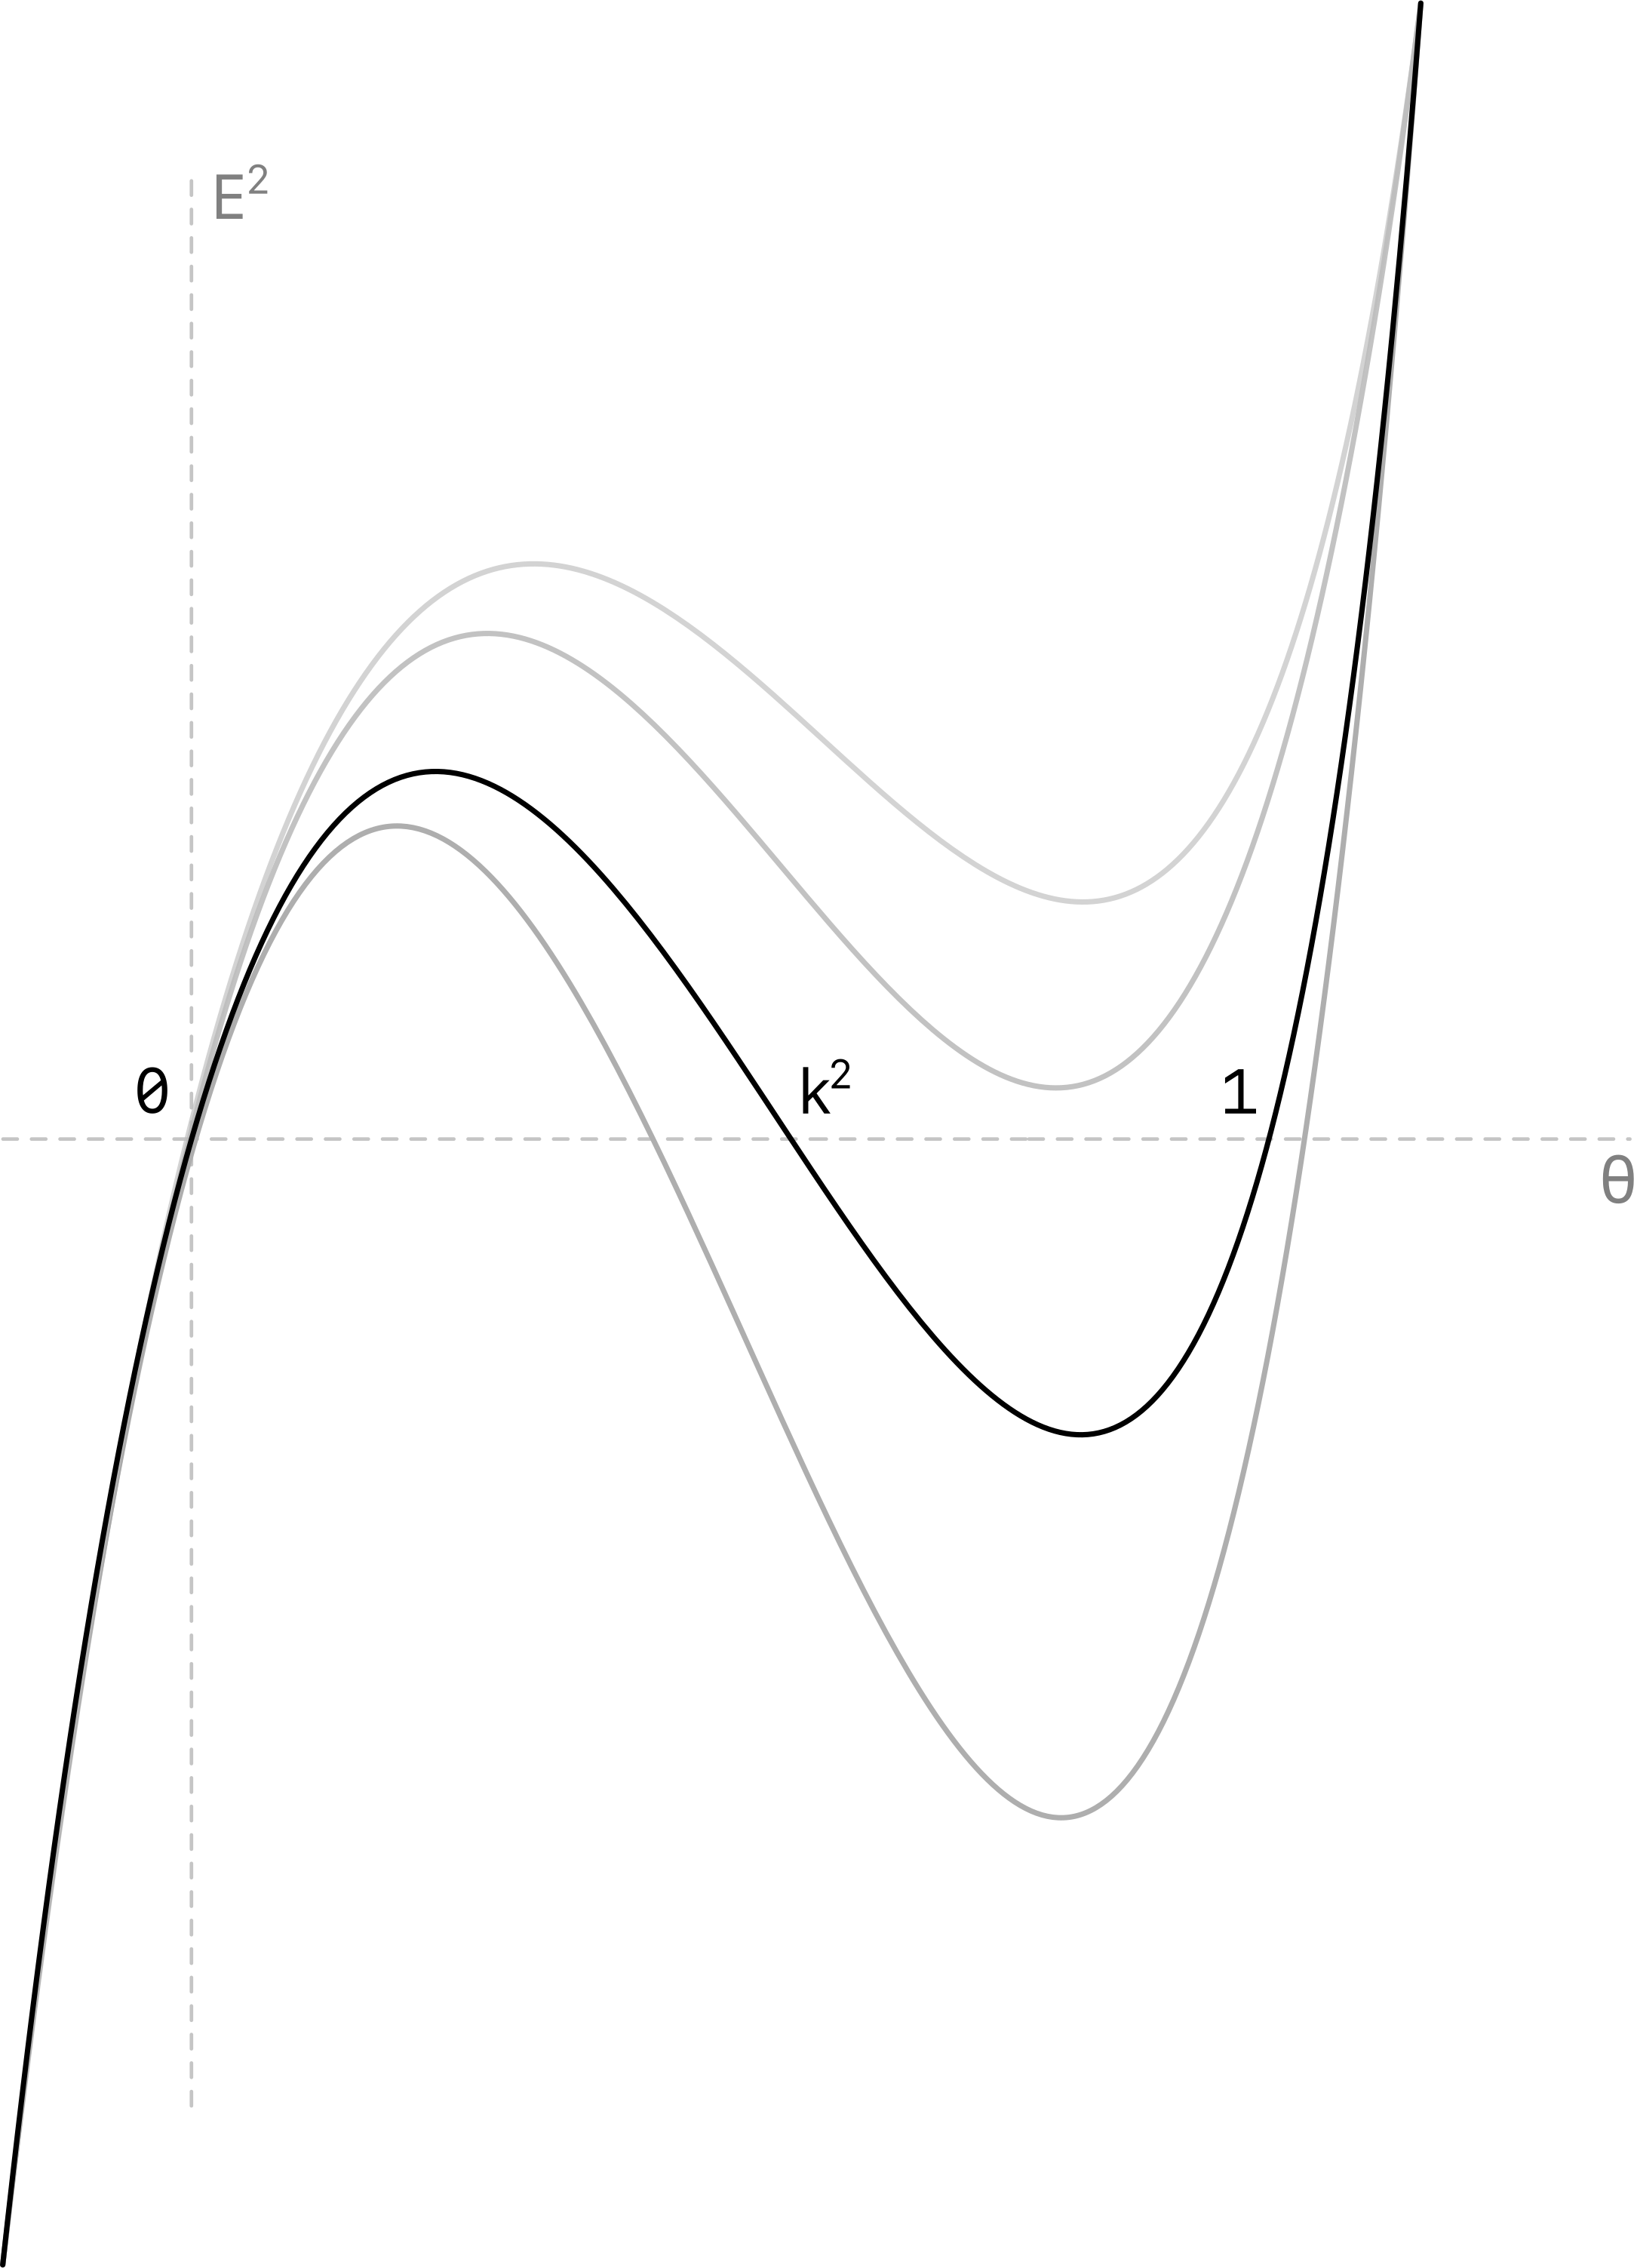
\includegraphics[width=60mm]{./img/ellipticSquare.png}\vspace{1mm}
    \captionof{figure}{\textls[-50]{\mono{Polynomial {E\textsuperscript{2}(\uptheta)} with one and three real root(s) in $\mathbb{R}$ space}}}
    \label{fig:ci}
  \end{minipage}
  \noindent
  \begin{minipage}{\linewidth}
    \centering
    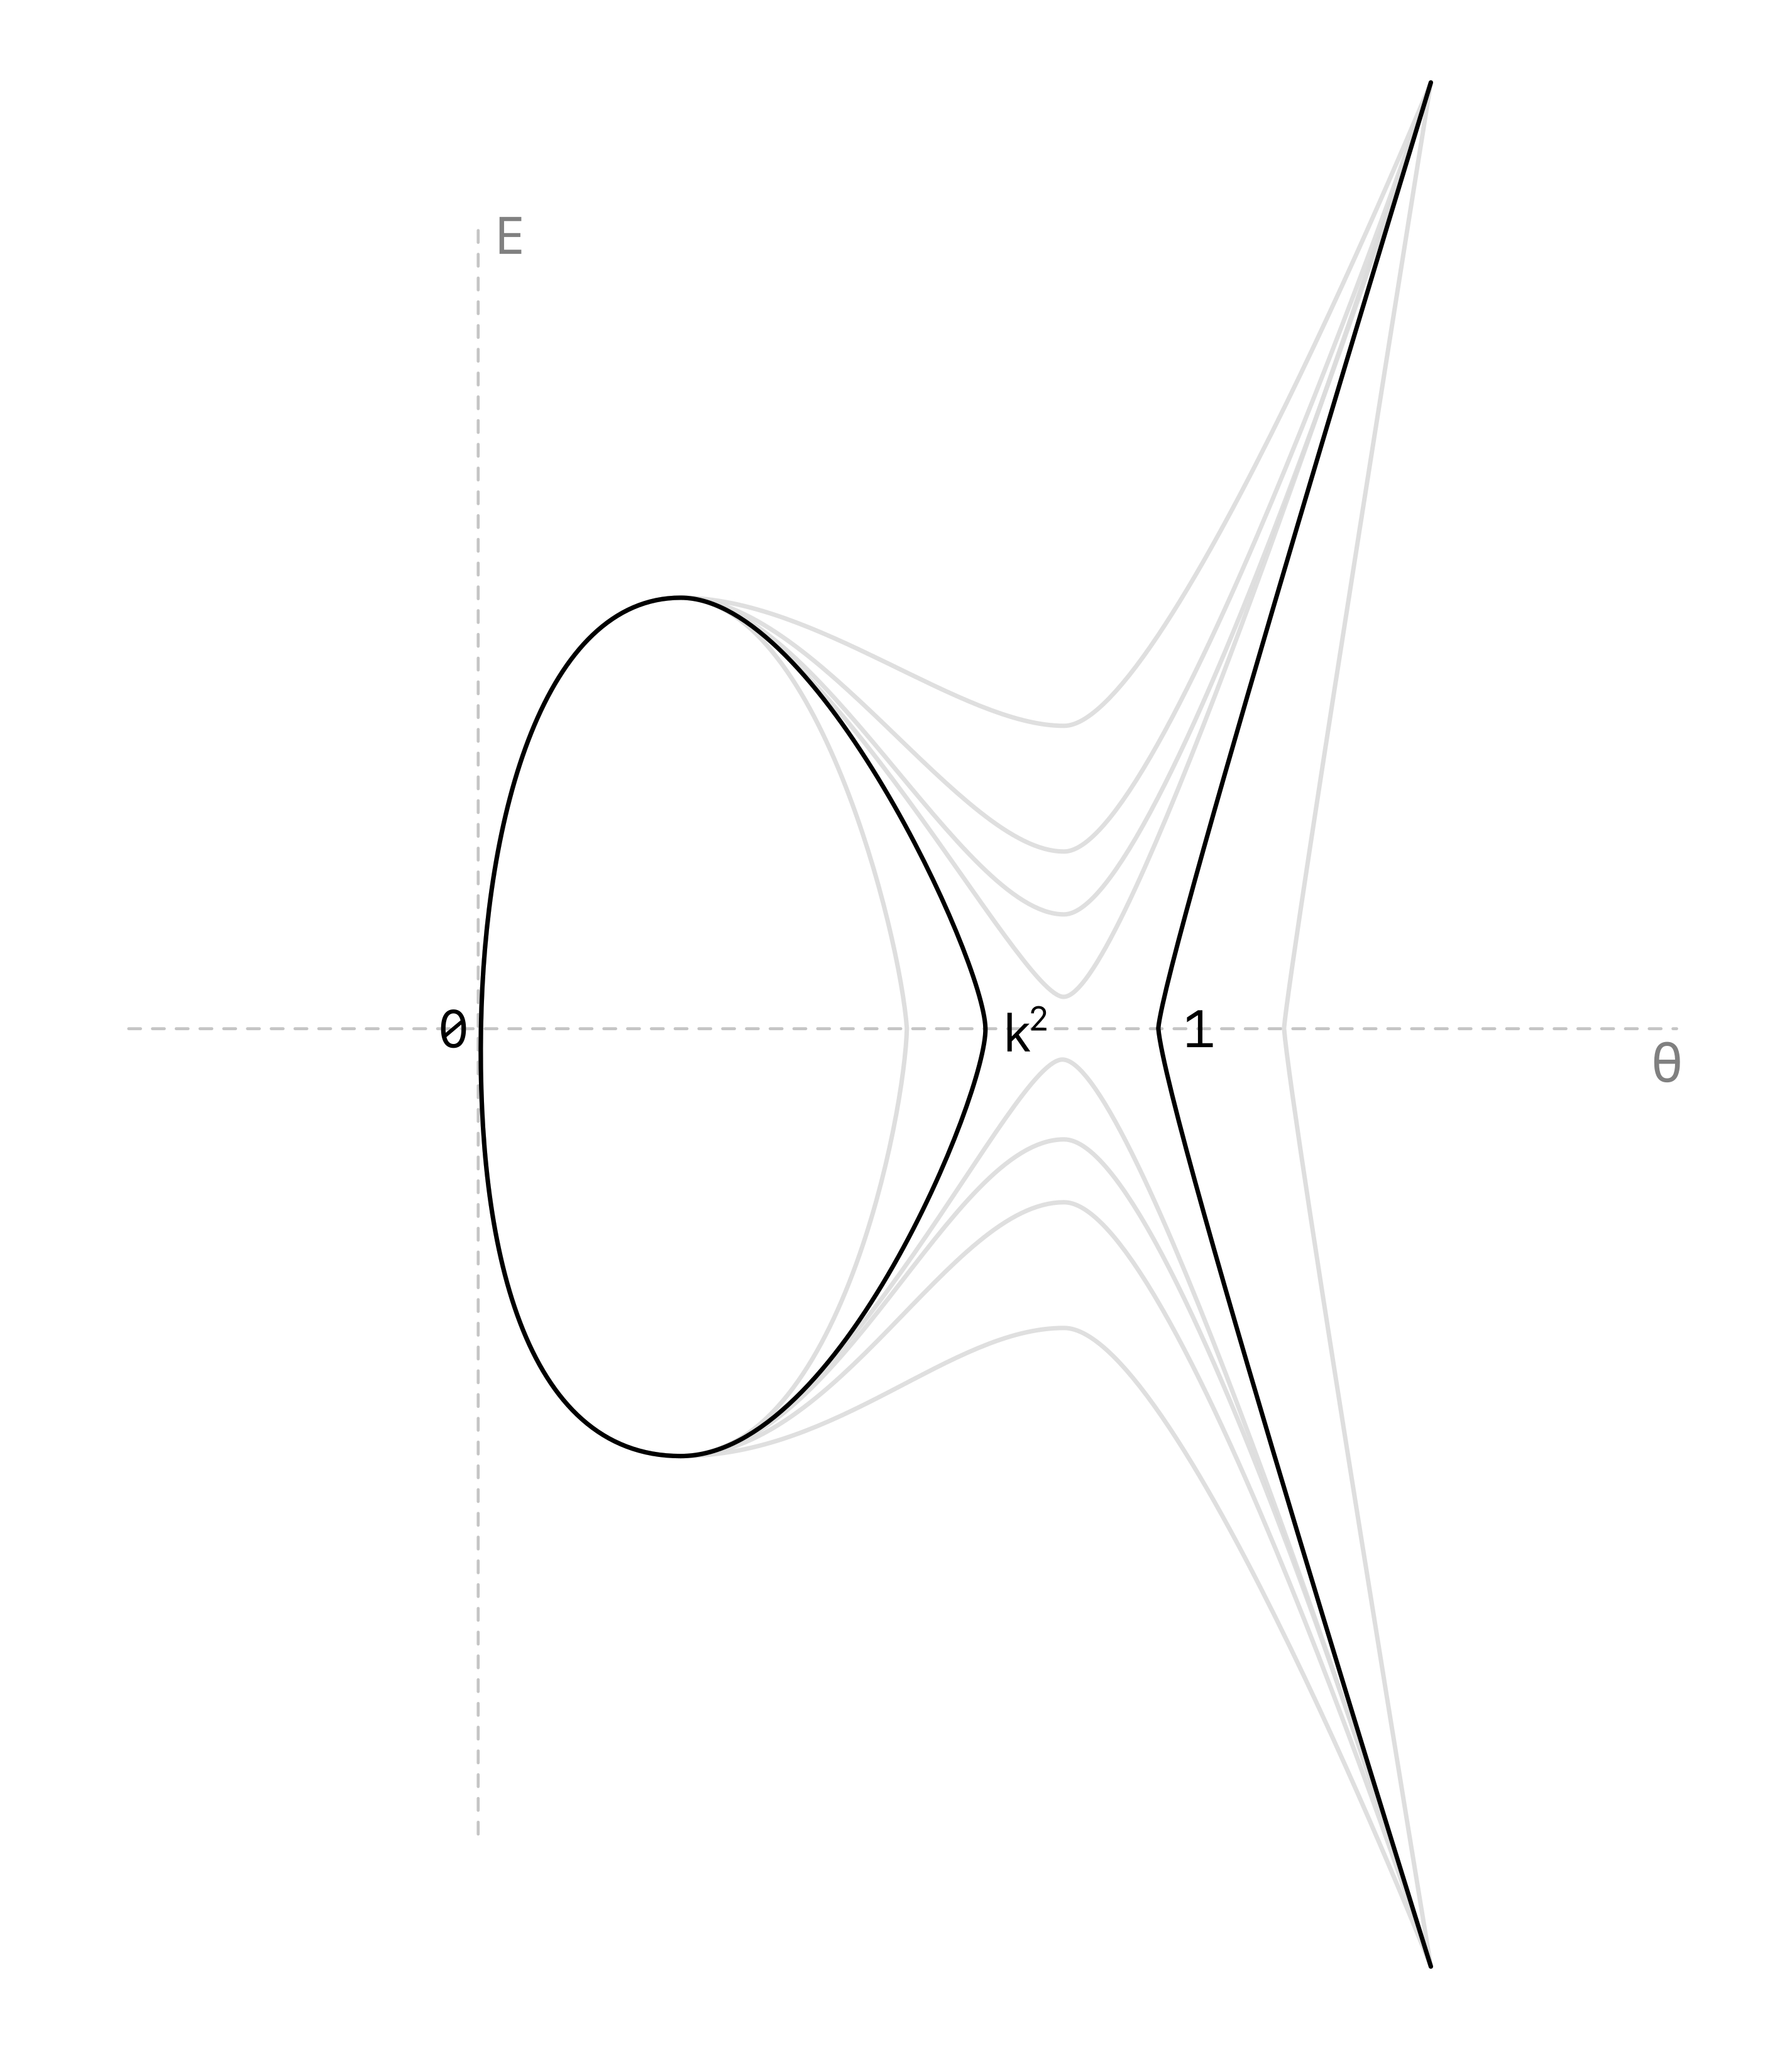
\includegraphics[width=60mm]{./img/ellipticCurve.png}\vspace{1mm}
    \captionof{figure}{\textls[-50]{\mono{Family of curves {E(\uptheta)} with one and three real root(s) in $\mathbb{R}$ space}}}
    \label{fig:ec}
  \end{minipage}
\end{multicols}
\begin{flushleft}
  \textls[-50]{\mono{
  \vspace{-5mm}
  \begin{center}
    {E\textsuperscript{2}(\uptheta)} = {\uptheta}\textsuperscript{3} + r\cdot\,{\uptheta}\textsuperscript{2} + p\,\cdot\,{\uptheta} + q,
  \end{center}
  \vspace{2mm}
  which is precisely the more familiar and recognisable form of the {\mbold{elliptic curve}}. Note that the form of {E({\uptheta})} in the above example asserts three roots of {E(\uptheta)}, i.e. 0, k\textsuperscript{2}, 1. This is however not true for generic elliptic curves which may have only one real root depending on the values of p, q and r, all of which are functions of k in return. In our particular example, r = -(1 + k\textsuperscript{2}), p = k\textsuperscript{2} and q = 0. Some readers may feel cheated at this point since we have just said that an elliptic curve is simply the square root of a cubic polynomial. This is indeed correct but not every cubic polynomial is an elliptic curve; the coefficients of the cubic polynomial must be such that there are no repeated roots, i.e. they represent a legitimate ellipse with legal values of e\textsuperscript{2} and k\textsuperscript{2}. Lastly, we note that the if the elliptic curve has 3 real roots, then evaluation of (4) requires integrating {E(\uptheta)} in the range (k\textsuperscript{2}, 1) where it is purely complex. In other words, figure \ref{fig:ec} doesn't paint the entire picture of elliptic curves with three real roots instead of one. To fully grasp the topological intuition behind {E(\uptheta)}, we must include the complex plane in our graphics. We also make a note of the abstract parameterisation {\uptheta} = 1 - e\textsuperscript{2}x\textsuperscript{2} that led to the easier form of the elliptic curve in (4); what led to this non-geometric choice?{\textsuperscript{\textcolor{blue}{Q1}}}
  \linebreak\linebreak\linebreak
  \textbf{\Large\pbold\textls[-25]{PERIODICITY}}\linebreak\linebreak
  It was Abel and Jacobi who first understood that the inverse of the intergal in (2a) is periodic and more relevant than the intergal itself, i.e.
  \vspace{2mm}
  \begin{center}
    F($\bar{\text{x}}$) = {{\raisebox{-1mm}{\huge\mate{^^^^222b}}}\textsuperscript{\raisebox{2.5mm}{\small{$\bar{\text{x}}$}}}}{\hspace{-2.5mm}\textsubscript{\raisebox{-2.5mm}{\footnotesize{0}}}}\;$\displaystyle\frac{\text{1}}{\text{(1 - x\textsuperscript{2})\textsuperscript{1/2}}}$\,{\resizebox{5px}{7px}{\updelta}}x = sin\textsuperscript{-1}($\bar{\text{x}}$), or
  \end{center}
  \begin{center}
    F({\upvarphi}) = {{\raisebox{-1mm}{\huge\mate{^^^^222b}}}\textsuperscript{\raisebox{2.5mm}{\upvarphi}}}{\hspace{-3mm}\textsubscript{\raisebox{-2.5mm}{\footnotesize{0}}}}\;{\resizebox{5px}{7px}{\updelta}}{\uptheta} = {\upvarphi},
  \end{center}
  \begin{flushright}
    {\vspace{-8mm}\mono{(5)}}
  \end{flushright}
  \vspace{2mm}
	when expressed using trigonometric parameterisation (x, y) {\rightarrow} (sin{\,\uptheta}, cos{\,\uptheta}). There are two interesting things to note here: a) F($\bar{\text{x}}$) is precisely equal to the argument {\upvarphi} of a sinusoid, and b) the argument {\upvarphi} of the sinusoid is precisely equal to the final geometric angle (in the limits of the integral) in parameterised coordinates. These precise observations and their generalisations in Jacobi's and Abel's works triggered several prominent number theorists to take note of elliptic integrals and their remarkable properties. For instance, the above integral becomes readily calculable only once we insert the parameterisation (x, y) = [{\large\pala\it{f}}\hspace{0.4mm}(\uptheta), {\large\pala\it{f}}\hspace{0.2mm}'\hspace{-1mm}(\uptheta)] {\rightarrow} (sin{\,\uptheta}, cos{\,\uptheta}). Based on this observation, Abel and Jacobi asserted that the key to decoding elliptic intergals is to find a similar parameterisation ({\large\pala\it{f}}\hspace{0.4mm}, {\large\pala\it{f}}\hspace{0.2mm}') which reduces the elliptic intergal to an integrable form. Thus the search had begun for such parameterisations, primarily by Jacobi and Abel at the beginning and later by Weistrausse. Legendre in the past had re-arranged equation (2) in another form which turned out to be more useful for Jacobi. Legendre's form of (2) simply reads
  \begin{center}
    C(e) = {4\resizebox{7.25px}{5.3px}{\upalpha}}\,{{\raisebox{-1mm}{\huge\mate{^^^^222b}}}\textsuperscript{\raisebox{2.5mm}{\footnotesize{1}}}}{\hspace{-2.5mm}\textsubscript{\raisebox{-2.5mm}{\footnotesize{0}}}}\;$\displaystyle\frac{\text{1 - e\textsuperscript{2}x\textsuperscript{2}}}{\text{[(1 - x\textsuperscript{2})(\text{1 - e\textsuperscript{2}x\textsuperscript{2}})]\textsuperscript{\textsuperscript{\scriptsize{1/2}}}}}$\,{\resizebox{5px}{7px}{\updelta}}x,
  \end{center}
  \begin{flushright}
    {\vspace{-8mm}\mono{(6)}}
  \end{flushright}
  \vspace{3mm}
  Legendre noted that integrating the elliptic integral of second kind is easier if one knows the integral evaluation of the first kind{\textsuperscript{\textcolor{blue}{2}}\blfootnote{\textls[-50]{\mono{\textsuperscript{2}{one can observe this by integrating (6) using the elementary 'by parts' formalism}}}}}, i.e. the same equation as above but with the numerator set to 1,
  \begin{center}
    F($\bar{\text{x}}$) = 4\resizebox{7.25px}{5.3px}{\upalpha}\,{{\raisebox{-1mm}{\huge\mate{^^^^222b}}}\textsuperscript{\raisebox{2.5mm}{\small{$\bar{\text{x}}$}}}}{\hspace{-2.5mm}\textsubscript{\raisebox{-2.5mm}{\footnotesize{0}}}}\;\;$\displaystyle\frac{\text{1}}{\text{[(1 - x\textsuperscript{2})(\text{1 - e\textsuperscript{2}x\textsuperscript{2}})]\textsuperscript{\textsuperscript{\scriptsize{1/2}}}}}$\,{\resizebox{5px}{7px}{\updelta}}x.
  \end{center}
  \begin{flushright}
    {\vspace{-8mm}\mono{(7)}}
  \end{flushright}
  \vspace{2mm}
  In parameterised form, elliptic integral of the first kind reads,
  \begin{center}
    F(e,\,\raisebox{0.25mm}{\resizebox{7.5px}{5px}{\upvarphi}}) = \,{{\raisebox{-1mm}{\huge\mate{^^^^222b}}}\textsuperscript{\raisebox{2.5mm}{\footnotesize{{{\upvarphi}}}}}}{\hspace{-3mm}\textsubscript{\raisebox{-2.5mm}{\footnotesize{0}}}}\;\;$\displaystyle\frac{\text{1}}{\text{(1 - e\textsuperscript{2}sin\textsuperscript{2}{\uptheta})\textsuperscript{1/2}}}$\,{\resizebox{5px}{7px}{\updelta}}{\uptheta},
  \end{center}
  \begin{flushright}
    {\vspace{-8mm}\mono{(8)}}
  \end{flushright}
  \vspace{2mm}
  which is eerily innocent-looking and quite similar to (3) except that the integrand is inverted. This particular form of the elliptic integral of the first kind is where Jacobi made the first meaningful step toward parameterising generic elliptic curves. Using nothing more than elementary geometry and trigonometry, Jacobi found F(e,\,\raisebox{0.25mm}{\resizebox{7.5px}{5px}{\upvarphi}}) to be analogous to the argument \resizebox{7.5px}{5px}{\upvarphi} of a sine-like (and cosine-like) function{\textsuperscript{\textcolor{blue}{2}}\blfootnote{\textls[-50]{\mono{\textsuperscript{2}{due to the said integral being literally equal to sin\textsuperscript{-1}(${\text{x}}$) for e = 0}}}}}, denoted by \resizebox{12px}{5.5px}{\kalam\textls[0]{sn}}\,${\text{F}}$, \resizebox{12px}{5.5px}{\kalam\textls[0]{cn}}\,${\text{F}}$, \resizebox{12.35px}{8.5px}{\kalam\textls[0]{dn}}\,${\text{F}}$ etc. Jacobi further evaluated that these bespoke sine- or cosine-like functions in fact have properties similar to a sinusoid such as periodicity. In fact, \resizebox{12px}{5.5px}{\kalam\textls[0]{sn}}\,${\text{F}}$, \resizebox{12px}{5.5px}{\kalam\textls[0]{cn}}\,${\text{F}}$, \resizebox{12.35px}{8.5px}{\kalam\textls[0]{dn}}\,${\text{F}}$ are all bi-periodic functions with complex periods in their argument F. In simpler words, \resizebox{12px}{5.5px}{\kalam\textls[0]{sn}} is doubly periodic with both periods ($\hat{\upomega}$\textsubscript{1},\,$\hat{\upomega}$\textsubscript{2}\;{$\in$}\;{$\mathbb{C}$}) being complex numbers, such that
  \vspace{2mm}
  \begin{center}
    \resizebox{12px}{5.5px}{\kalam\textls[0]{sn}}(F) = \resizebox{12px}{5.5px}{\kalam\textls[0]{sn}}(F + n\textsubscript{1}\,\cdot\,$\hat{\upomega}$\textsubscript{1}) = \resizebox{12px}{5.5px}{\kalam\textls[0]{sn}}(F + n\textsubscript{2}\,\cdot\,$\hat{\upomega}$\textsubscript{2}), and so on,
  \end{center}
  \begin{flushright}
    {\vspace{-7mm}\mono{(9)}}
  \end{flushright}
  \vspace{2mm}
  where $\hat{\upomega}$\textsubscript{1} and $\hat{\upomega}$\textsubscript{2} must necessarily be linearly-independent in {$\mathbb{R}$}, aka they are not mutually related by $\hat{\upomega}$\textsubscript{1}\,{\robot{^^^^2260}}\;{$\mathbb{R}$}\,\cdot\,$\hat{\upomega}$\textsubscript{2}. This however wasn't the most important assertion; Jacobi further found that no single-variable function could possibly have more than two independent complex periods, and all except elliptic integrals of the first and second (and third) kind have at most one independent period only. This was arguably the first solid proof that elliptic integrals were a special class of functions.\linebreak\linebreak
	These new set of functions \resizebox{12px}{5.5px}{\kalam\textls[0]{sn}}\,${\text{F}}$, \resizebox{12px}{5.5px}{\kalam\textls[0]{cn}}\,${\text{F}}$, \resizebox{12.35px}{8.5px}{\kalam\textls[0]{dn}}\,${\text{F}}$ soon came to be known as Jacobi's elliptic functions (read: Jacobi's generalised and redefined trigonometric functions). Jacobi's elliptic functions are generalisations of generic sine and cosine functions (which are traditionally defined on a circle) on an elliptic path. To understand this, consider that for any point (x, y) on a carterian surface, we may readily define the basic trigonometric functions as per our education to be 
  \begin{center}
    sin\,{\uptheta} = $\displaystyle\frac{\text{x}}{{\text{r}}}$ and cos\,{\uptheta} = $\displaystyle\frac{\text{y}}{{\text{r}}}$.
  \end{center}
  This definition relies on the assumption that (x\textsuperscript{2} + y\textsuperscript{2})\textsuperscript{1/2} = r is a constant equal to the radius of the circle on which the trigonometry is defined. Jacobi's elliptic functions extend these definitions to a generic path r(\uptheta) other than a circle. In addition, Jacobi's elliptic functions are not dependent on the geometrical angle {\resizebox{7.5px}{5px}{\upvarphi}} explicitly, but instead are a function of a redefined and abstract (= non-geometric) argument \resizebox{6px}{5.2px}{\upmu}, which is equal to {\resizebox{7.5px}{5px}{\upvarphi}} for a circle. For the particular case of an elliptic path, \resizebox{6px}{5.2px}{\upmu} can be evaluated by considering equation (8) along with the implied equivalence to equation (5) such that
  \begin{center}
    \resizebox{6px}{5.2px}{\upmu}\;\;\equiv\;\;F(e,\,\raisebox{0.25mm}{\resizebox{7.5px}{5px}{\upvarphi}}) = \,{{\raisebox{-1mm}{\huge\mate{^^^^222b}}}\textsuperscript{\raisebox{2.5mm}{\footnotesize{\hspace{-0.10mm}{\upvarphi}}}}}{\hspace{-3mm}\textsubscript{\raisebox{-2.5mm}{\hspace{-0.15mm}\footnotesize{0}}}}\;r(\uptheta,\,e)\,{\resizebox{5px}{7px}{\updelta}}{\uptheta} {\victr{^^^^2260}} \raisebox{0.25mm}{\resizebox{7.5px}{5px}{\upvarphi}}, where
  \end{center}
  \begin{center}
    r\;\;\equiv\;\;r(\uptheta,\,e) = $\displaystyle\frac{\text{1}}{\text{(1 - e\textsuperscript{2}sin\textsuperscript{2}{\uptheta})\textsuperscript{1/2}}}$
  \end{center}
  \begin{flushright}
    {\vspace{-8mm}\mono{(11)}}
  \end{flushright}
  \vspace{2mm}
  Like previously stated, \resizebox{6px}{5.2px}{\upmu} is an abstract redefinition of the argument (geometric angle) of regular trigonometric functions, to allow them to work with Jacobi's elliptic functions, such that \resizebox{6px}{5.2px}{\upmu} = {\resizebox{7.5px}{5px}{\upvarphi}} is a special case of a circle. Consequently, Jacobi's functions are simple redefinitions of sin\,{\resizebox{7.5px}{5px}{\upvarphi}} and cos\,{\resizebox{7.5px}{5px}{\upvarphi}} to \resizebox{12px}{5.5px}{\kalam\textls[0]{sn}}\,\resizebox{6px}{5.2px}{\upmu} and \resizebox{12px}{5.5px}{\kalam\textls[0]{cn}}\,\resizebox{6px}{5.2px}{\upmu}, along with a third function \resizebox{12.35px}{8.5px}{\kalam\textls[0]{dn}}\,\resizebox{6px}{5.2px}{\upmu} that captures the variation in r(\uptheta). These redefined trigonometric functions are more general in nature and a circle is a special case of this general topology; in case of a circle, this topology reduces \resizebox{12px}{5.5px}{\kalam\textls[0]{sn}}, \resizebox{12px}{5.5px}{\kalam\textls[0]{cn}} and \resizebox{12.35px}{8.5px}{\kalam\textls[0]{dn}} to sine, cosine and 1 respecitvely.
  \begin{center}
    \resizebox{12px}{5.5px}{\kalam\textls[0]{sn}}\,\resizebox{6px}{5.2px}{\upmu} = $\displaystyle\frac{\;\;\text{x\textsubscript{i}}}{{\text{\upgamma}}}$ = $\displaystyle\frac{\;\;\text{x}}{{\text{r(\uptheta,\,e)}}}$,
  \end{center}
  \begin{center}
    \resizebox{12px}{5.5px}{\kalam\textls[0]{cn}}\,\resizebox{6px}{5.2px}{\upmu} = $\displaystyle\frac{\;\;\text{y\textsubscript{i}}}{{\text{\upgamma}}}$
  \end{center}
  \begin{center}
    \resizebox{12.35px}{8.5px}{\kalam\textls[0]{dn}}\,\resizebox{6px}{5.2px}{\upmu} = $\displaystyle\frac{\text{\upgamma}}{{\text{r(\uptheta,\,e)}}}$
  \end{center}
  \begin{flushright}
    {\vspace{-8mm}\mono{(10)}}
  \end{flushright}
  \vspace{2mm}
  There are two explicit differences to note when comparing Jacobi's elliptic functions to the traditional trigonometric functions: a) first is the appearance of a third elliptic function \resizebox{12.35px}{8.5px}{\kalam\textls[0]{dn}} capturing the curvature of the path, and b) second is the change in argument from geometric {\resizebox{7.5px}{5px}{\upvarphi}} to non-geometric \resizebox{6px}{5.2px}{\upmu}.\linebreak\linebreak  
  Jacobi noted that the trajectory (aka topology) of an ellipse is completely described by two concentric circles that inscribe (radius \raisebox{0.25mm}{\resizebox{6.5px}{5px}{\upgamma}} = 1) and circumscribe (radius {\resizebox{7.25px}{5.3px}{\upalpha}}) the ellipse, and Jacobi's trigonomatric functions capture the projection of the ellipse (encased by the two circles) onto these two circles; these two circles is some sense form the basis of the elliptic topology. This geometric interpretation of Jacobi's functions is shown in figures \ref{fig:jacobi} and \ref{fig:dual}.\linebreak
  }}
\end{flushleft}
\begin{multicols}{2}
  \noindent
  \begin{minipage}{\linewidth}
    \centering
    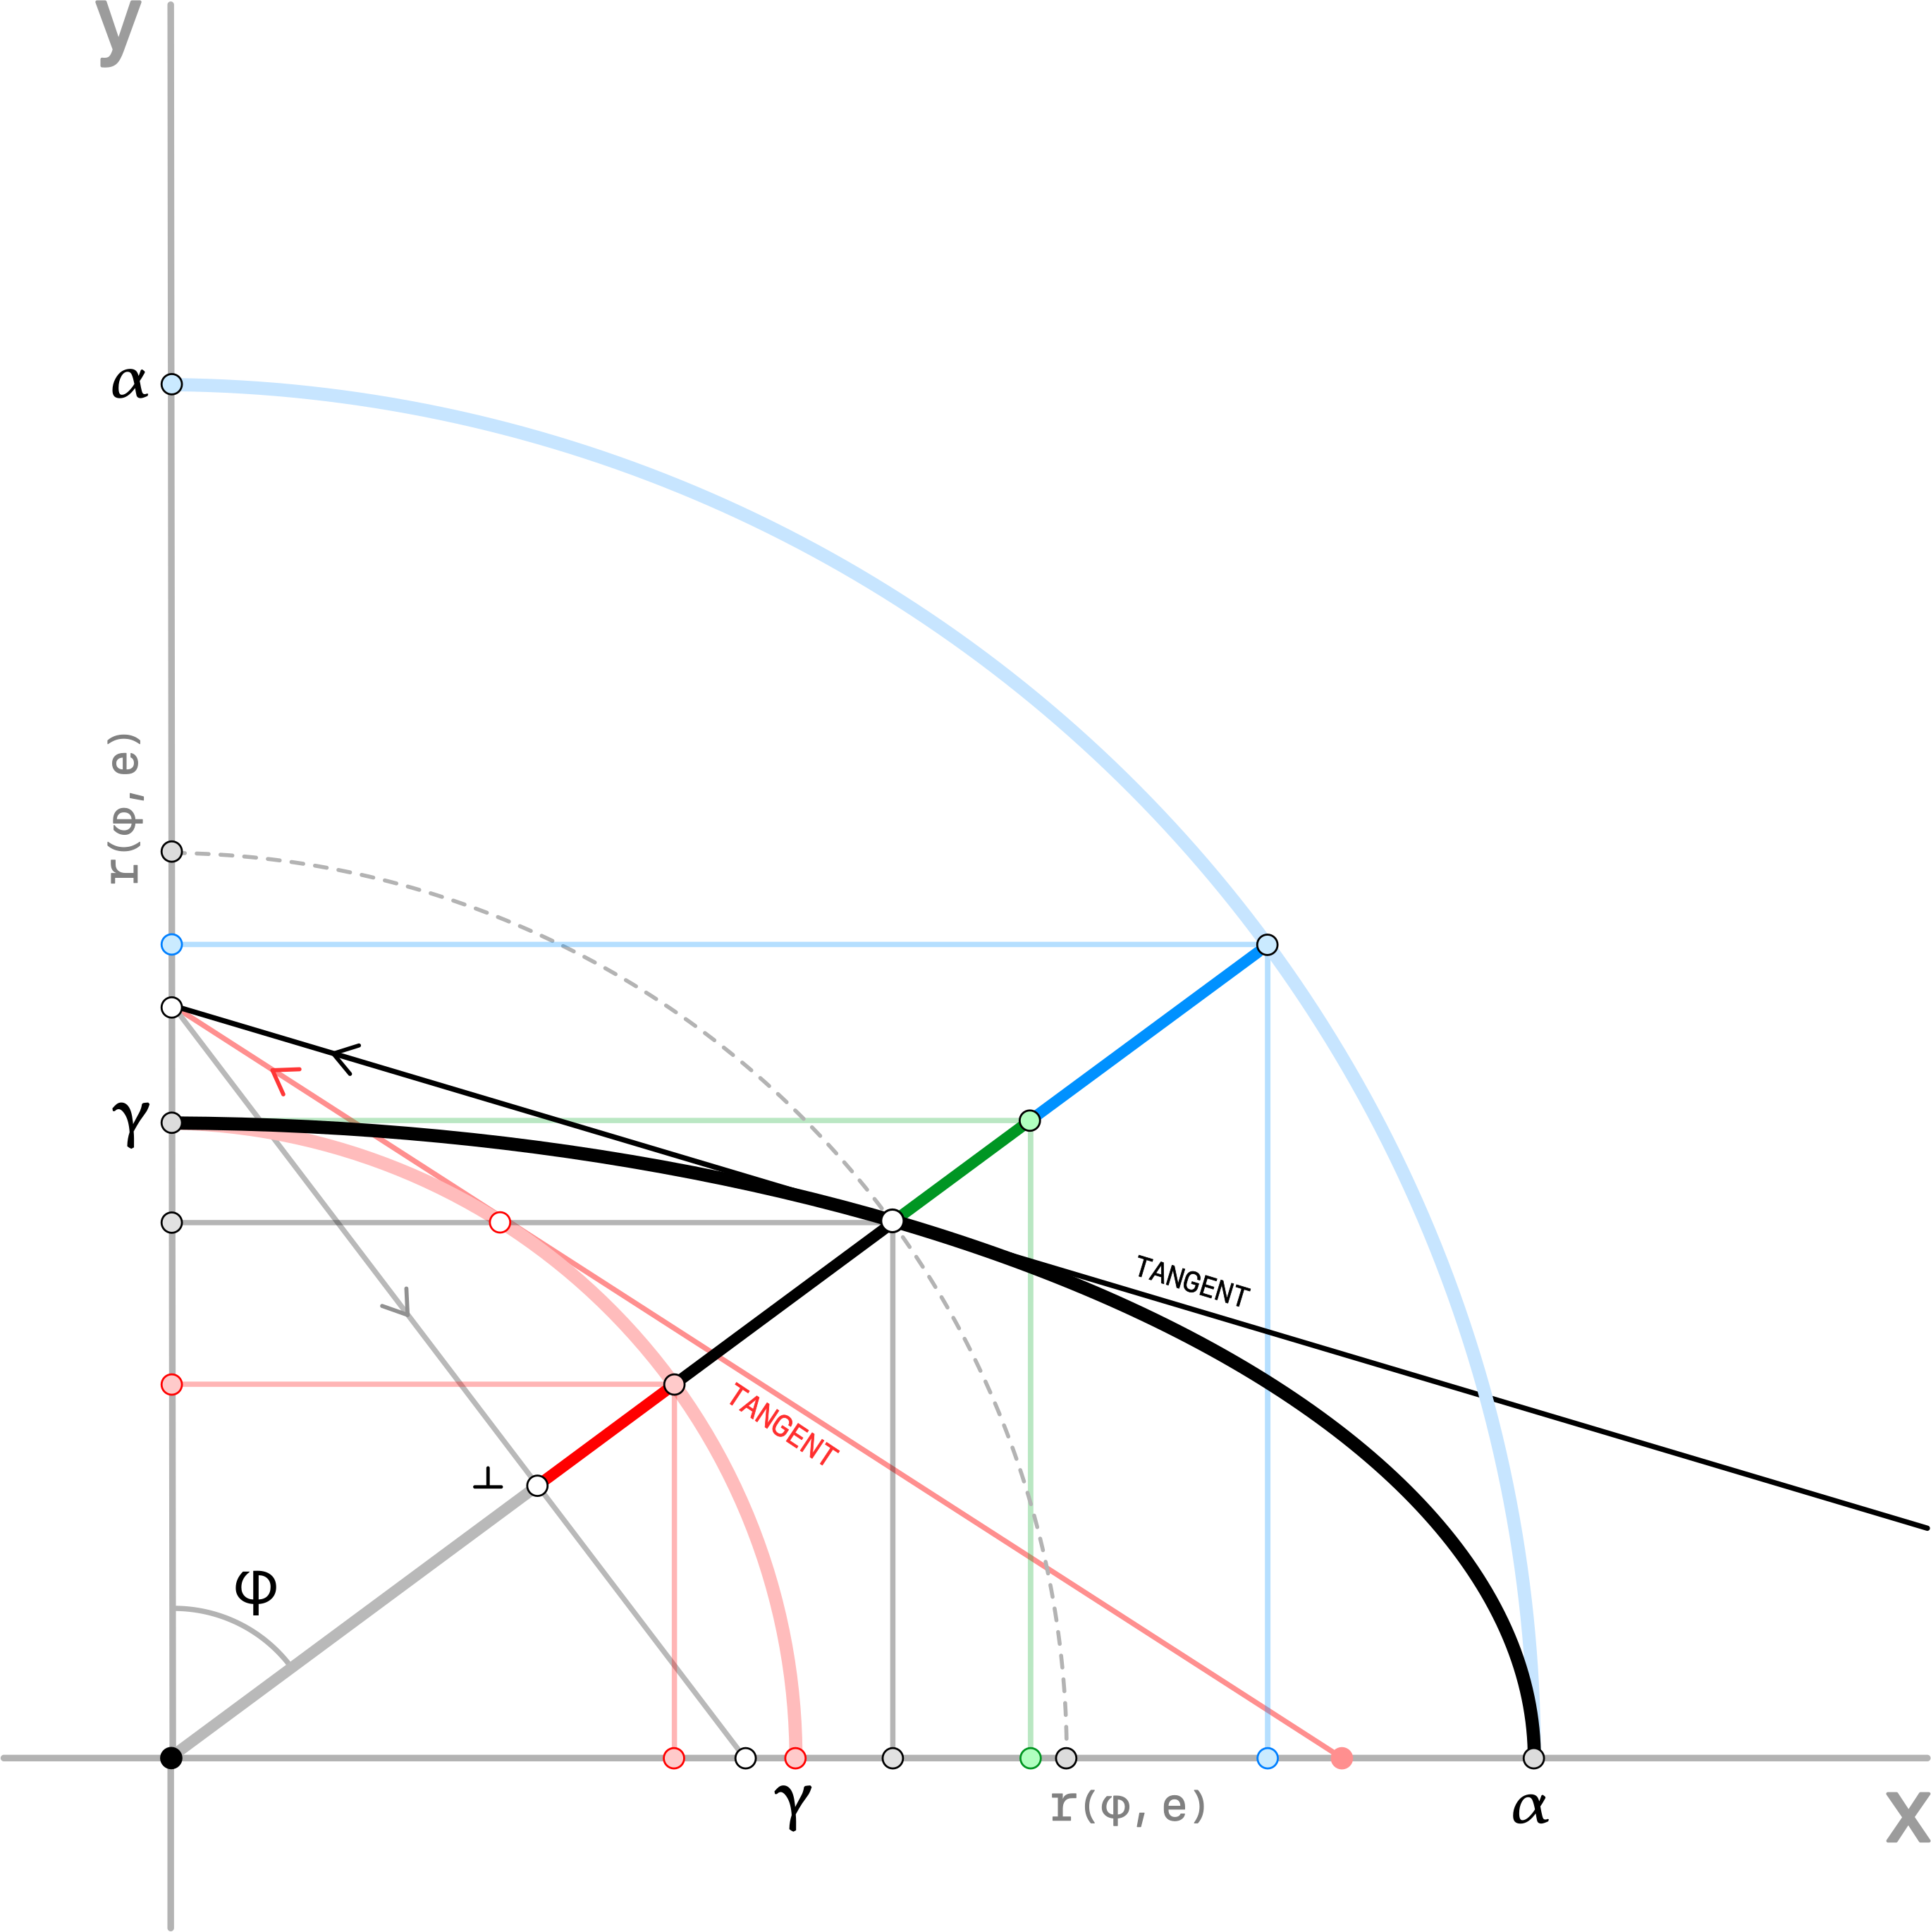
\includegraphics[width=77.5mm]{./img/jacobiSine.png}\vspace{1mm}
    \captionof{figure}{\textls[-50]{\mono{Jacobi's elliptic trigonometric functions}}}
    \label{fig:jacobi}
  \end{minipage}
  \noindent
  \begin{minipage}{\linewidth}
    \centering
    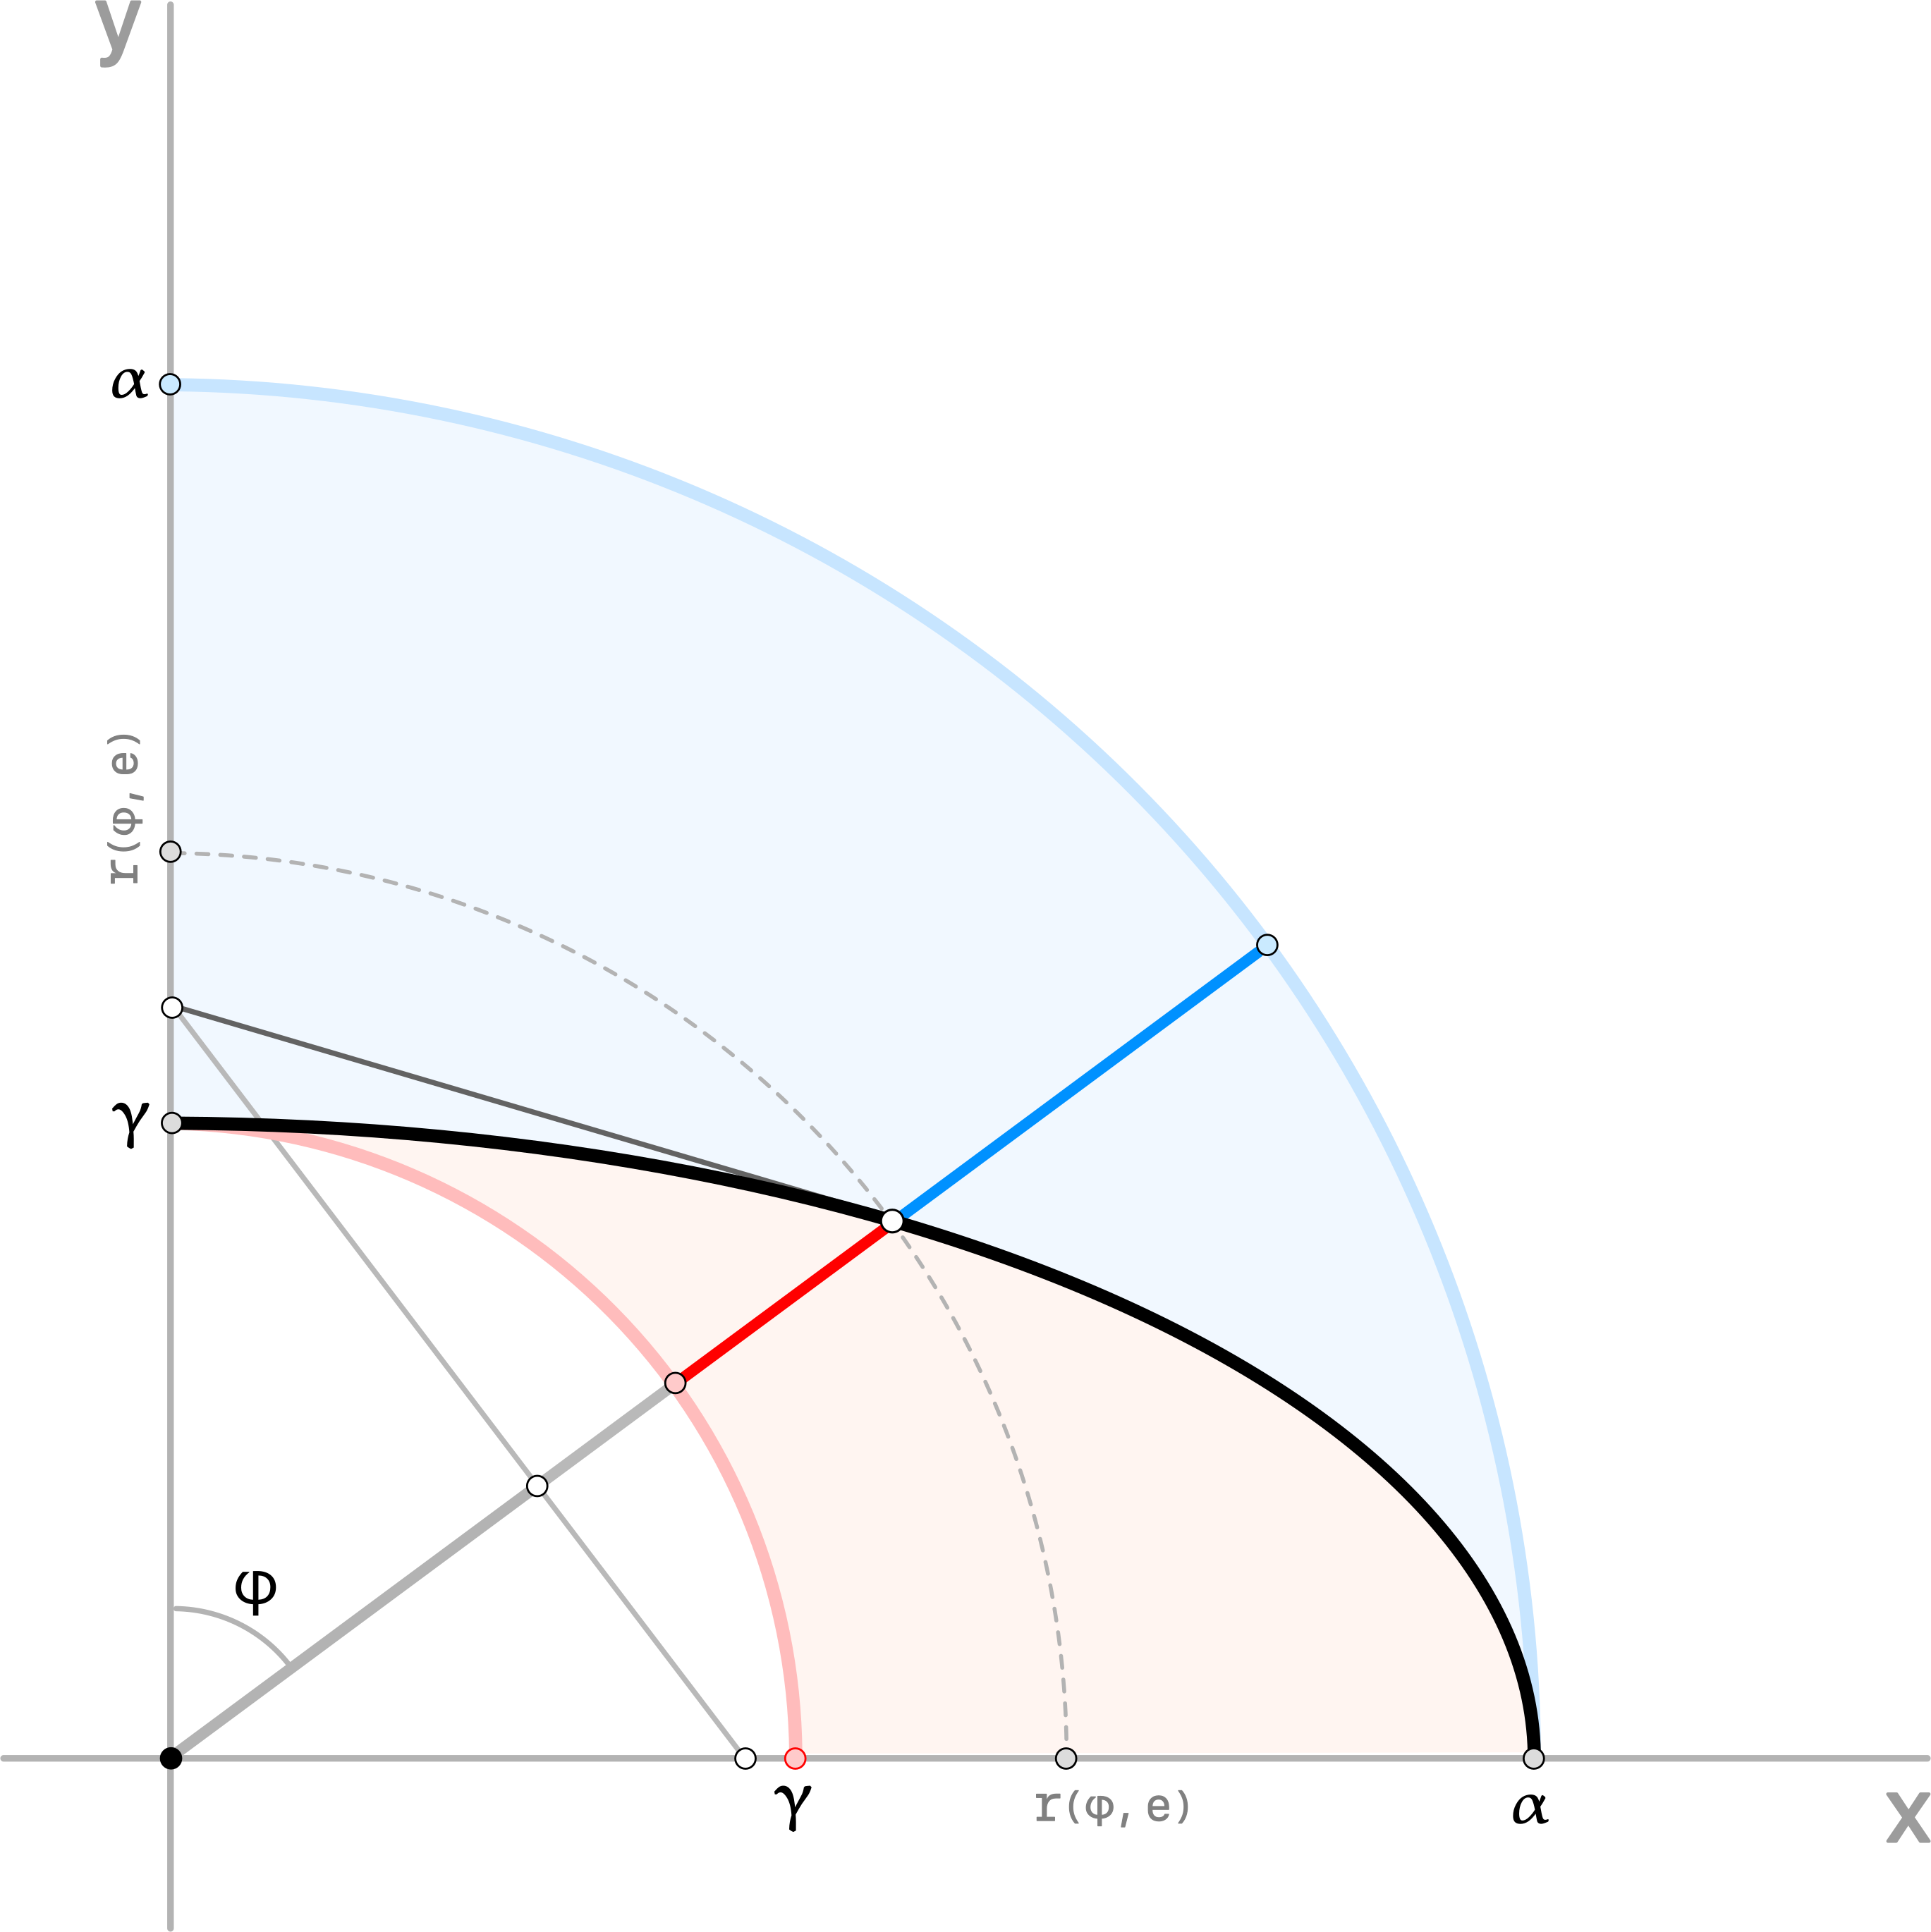
\includegraphics[width=77.5mm]{./img/dualTopology.png}\vspace{1mm}
    \captionof{figure}{\textls[-50]{\mono{Split topology for ellipses underlying Jacobi's trigonometry}}}
    \label{fig:dual}
  \end{minipage}
\end{multicols}
\vspace{2mm}
\begin{flushleft}
  \textbf{\Large\pbold\textls[-25]{COMPLEX BI-PERIODICITY}}\linebreak\linebreak
  \textls[-50]{\mono{We are now at a point where we cannot avoid complex numbers any further. We faced them while trying to evaluate the elliptic integral when {E($\uptheta$)} had three real roots, and now we are facing them yet again when trying to retrace Jacobi's steps. In order to understand the topology of Jacobi's trigonometric functions, we must first introduce complex numbers and particularly n-dimensional lattices in complex space, both of which are necessary to understand bi-periodic functions with complex periods.\linebreak\linebreak
  Periodicity in real space $\mathbb{R}$ is simple to understand topologically. Complex numbers on the other hand behave as vectors in geometrical sense, and therefore periodicity in a vector space must be understood. For example, consider equation (9) defining periodicity in complex space with periods $\hat{\upomega}$\textsubscript{1} and $\hat{\upomega}$\textsubscript{2}. Consider any one of the periods $\hat{\upomega}$\textsubscript{1} to begin with and calculate a few iterations of of $\bar{\text{x}}$ + n\textsubscript{1}\,\cdot\,$\hat{\upomega}$\textsubscript{1} for a few values of n\textsubscript{1} = 1, 2,\;...\;6. We find that the corresponding vectors all lie on a straight line in the complex plane parallel to $\hat{\upomega}$\textsubscript{1}; these points are shown in figure 3 with their indices. In the same way, the vectors associated with the second period also generate a straight line with a different slope parallel to $\hat{\upomega}$\textsubscript{2}. The two sets of points lying on lines of unequal slope in the complex plane form a lattice, denoted by $\hat{\upomega}$\textsubscript{1}\,{\times}\;$\hat{\upomega}$\textsubscript{2}, such that the bi-periodic function is also periodic on the lattice. The trivial extension of this is that when both periods are linearly-dependent, the lattice is in fact just a straight line. Recall that for a mono-periodic real functions such as sin(x), its parameterised form is a closed curve (a circle). In other words, a mono-periodic function parameterises to a closed curve in 2-dimensional space. In the same way, a bi-periodic function parameterises to a closed surface in 3-dimensional space. Does this mean that a bi-periodic C($\bar{\text{x}}$) is a closed surface in complex hyperplane{\textsuperscript{\textcolor{blue}{2}}\blfootnote{\textls[-50]{\mono{\textsuperscript{2}{Hyperplane refers to the (N + 1)-dimensional space that parameterises the periodic N-dimensional function}}}}}? Yes. How does this surface look? Figure 4 shows a visualisation of the parameterisation similar to how a circle can be obtained by parameterising a sinusoid by \resizebox{5.5px}{7px}{\uptheta}. The form of a bi-periodic C($\bar{\text{x}}$) is a complex torus, the only closed surface capable of bi-periodicity in three dimensions. It can be intuitively derived by rolling the lattice sheet into a cylinder along $\hat{\upomega}$\textsubscript{1}, and then joining the opposite ends of the rolled cylinder (by 'rolling' the cylinder second time along $\hat{\upomega}$\textsubscript{2}) to form a torus.
  }}
\end{flushleft}
\vspace{2mm}
\begin{multicols}{2}
  \noindent
  \begin{minipage}{\linewidth}
    \centering
    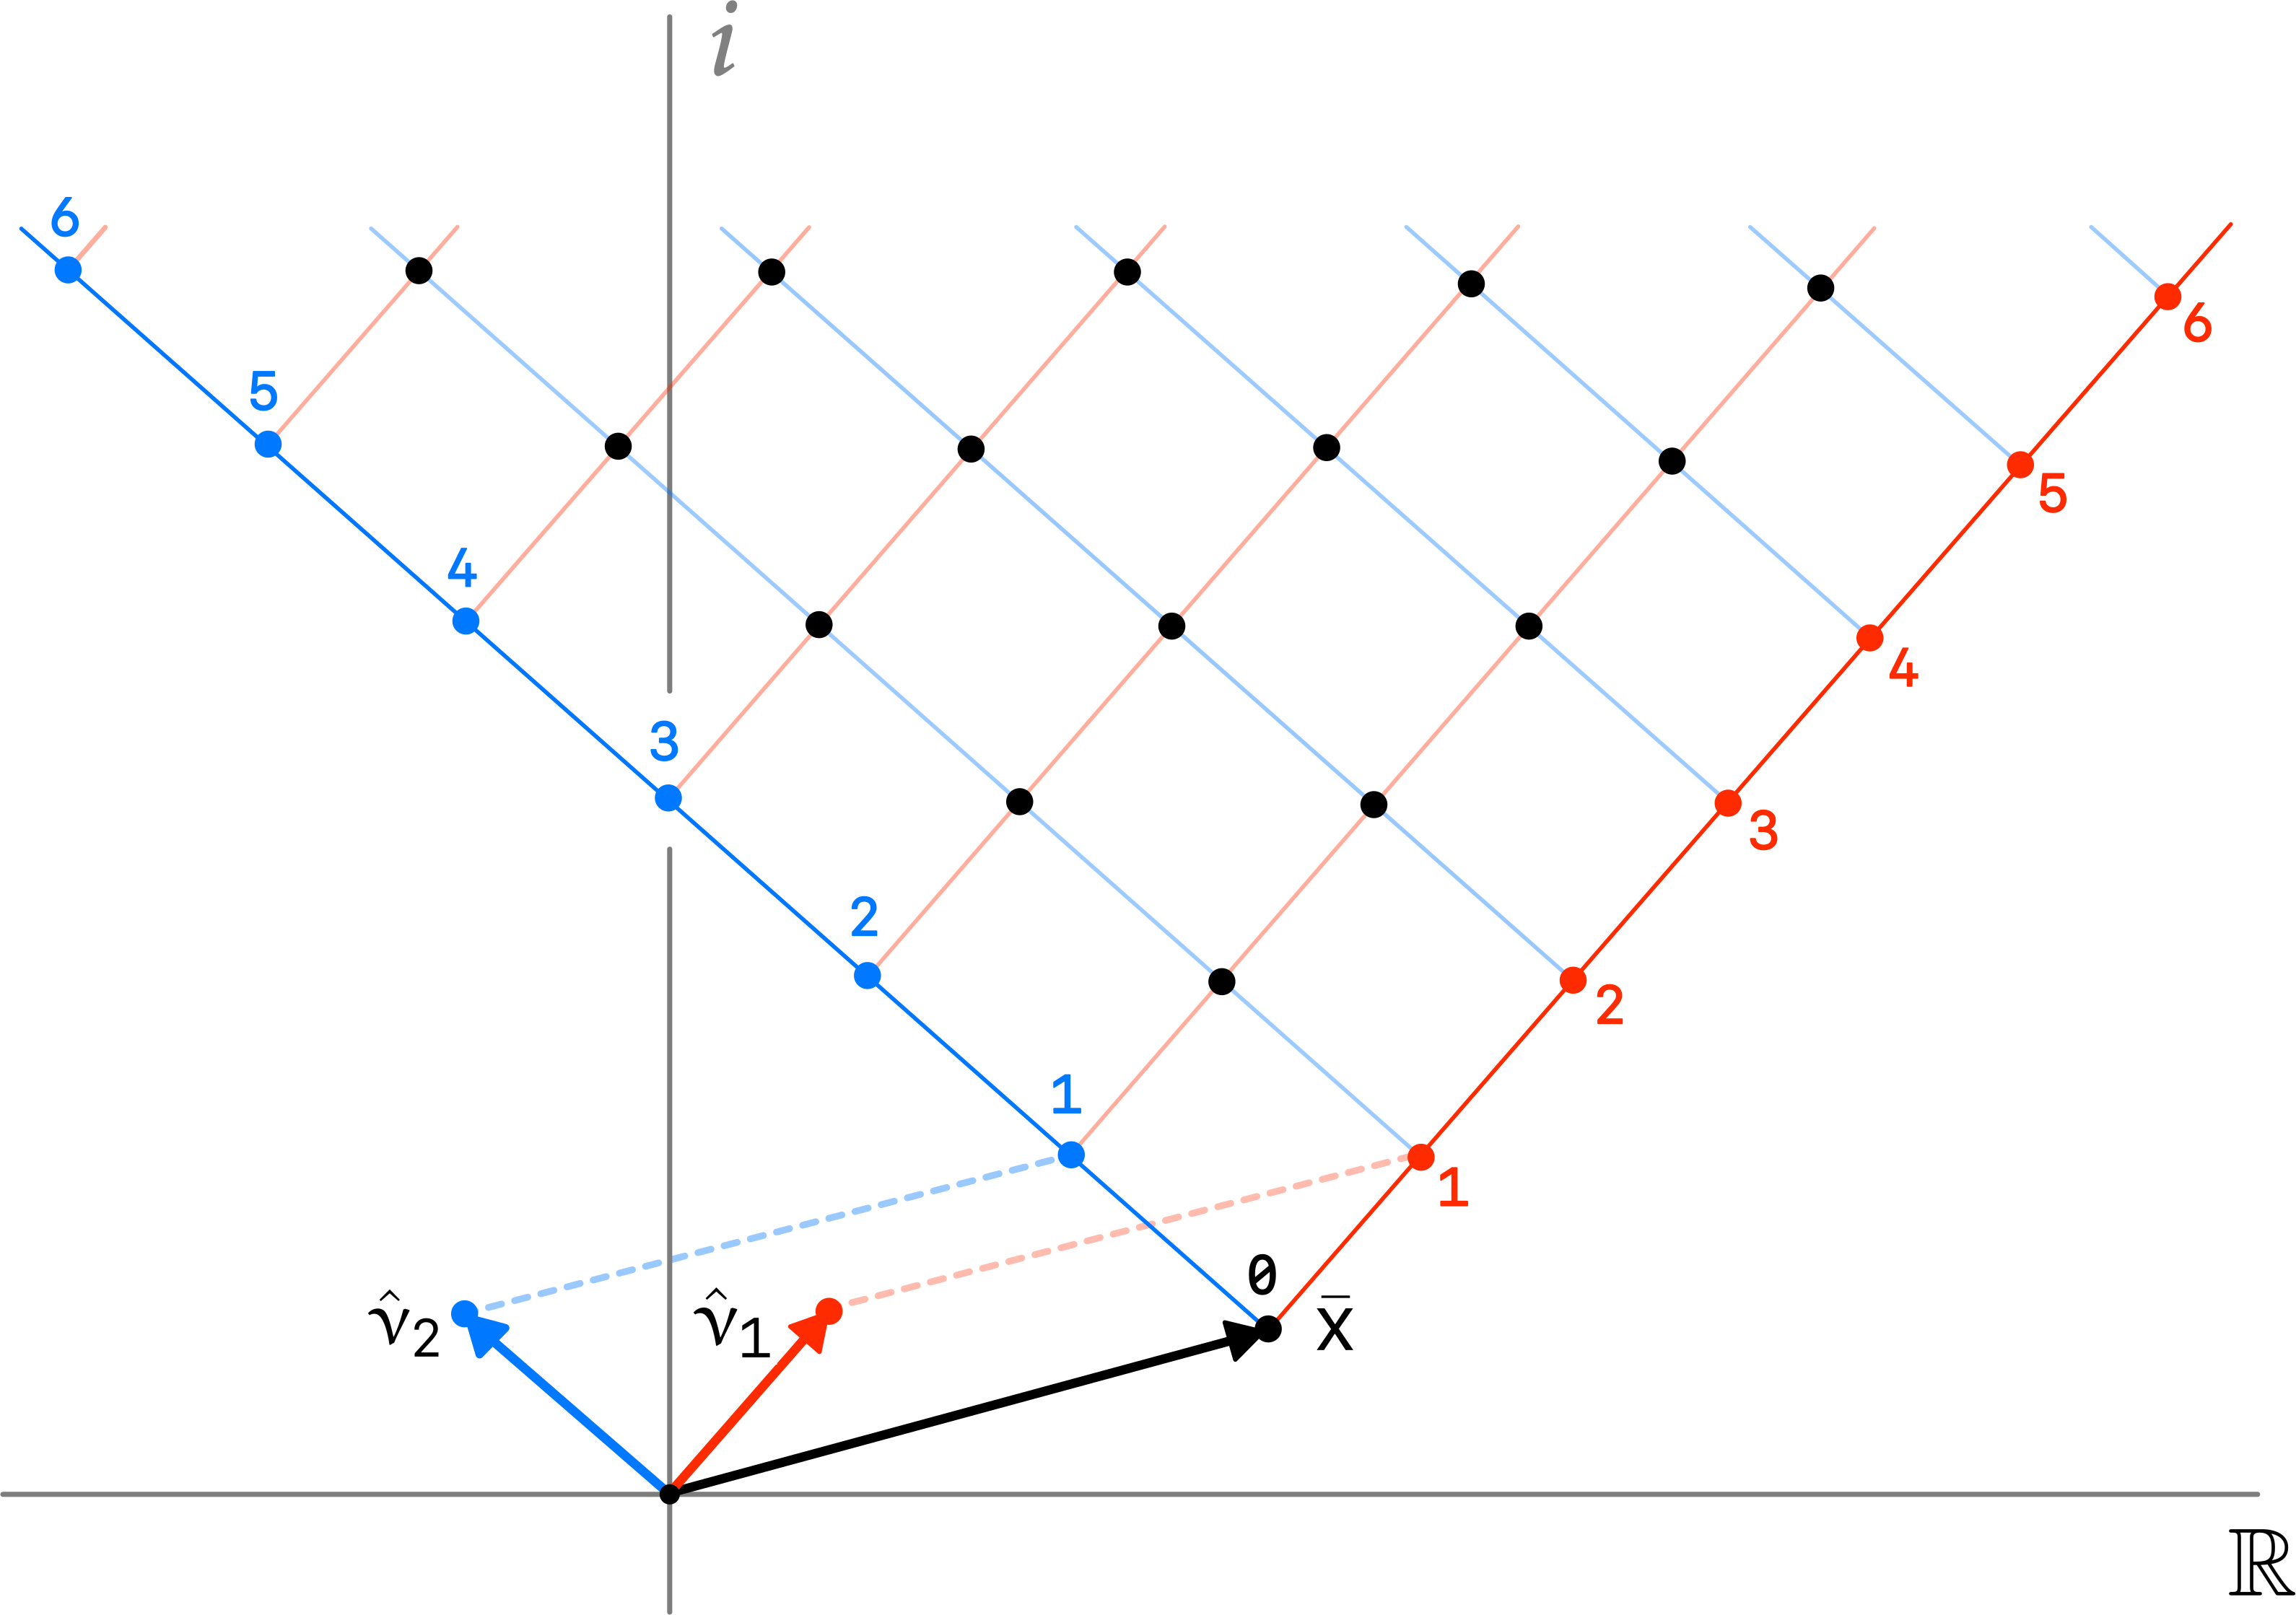
\includegraphics[width=75mm]{./img/complexBiPeriods.png}\vspace{1mm}
    \captionof{figure}{\textls[-50]{\mono{Complex lattice generated by a bi-periodic function with two linearly independent complex periods}}}
    \label{fig:ci}
  \end{minipage}
  \noindent
  \begin{minipage}{\linewidth}
    \centering
    \vspace{5.6mm}
    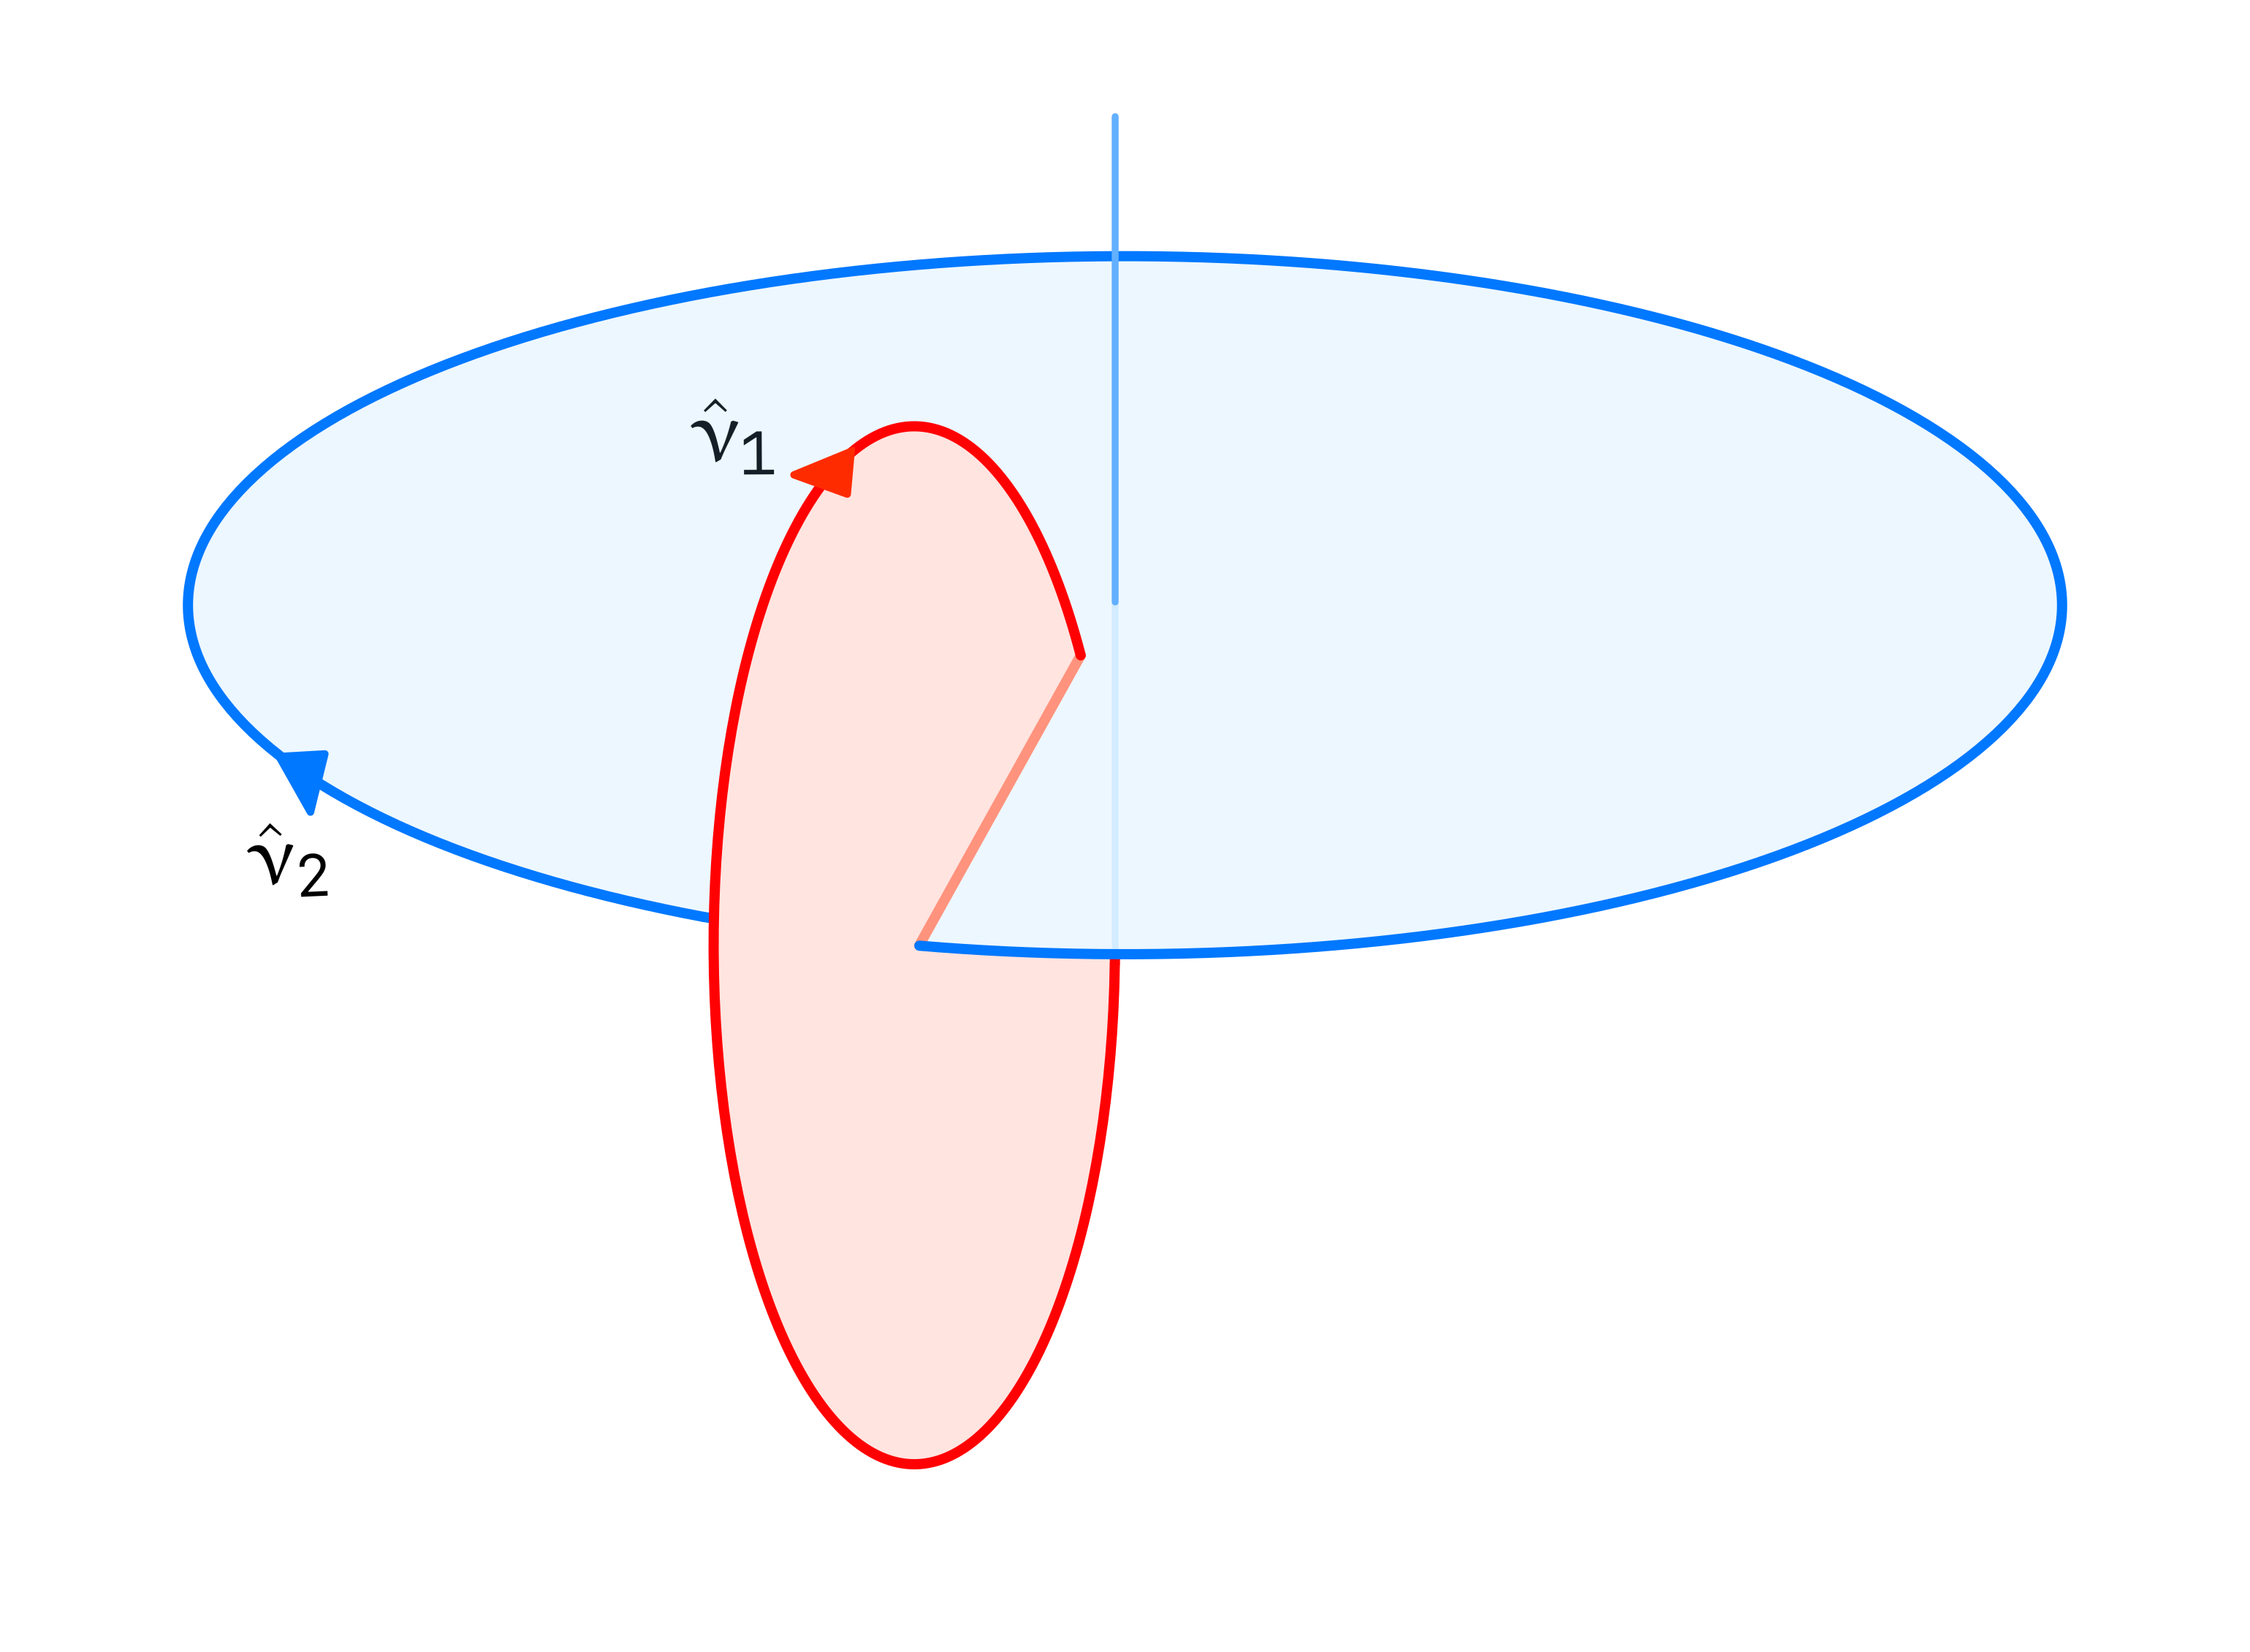
\includegraphics[width=59.1mm]{./img/complexTorus.png}\vspace{5.6mm}
    \captionof{figure}{\textls[-50]{\mono{Toroidal parameterisation of a complex lattice generated by a bi-periodic function}}}
    \label{fig:ec}
  \end{minipage}
\end{multicols}
\vspace{1mm}
\begin{multicols}{2}
  \noindent
  \begin{minipage}{\linewidth}
    \centering
    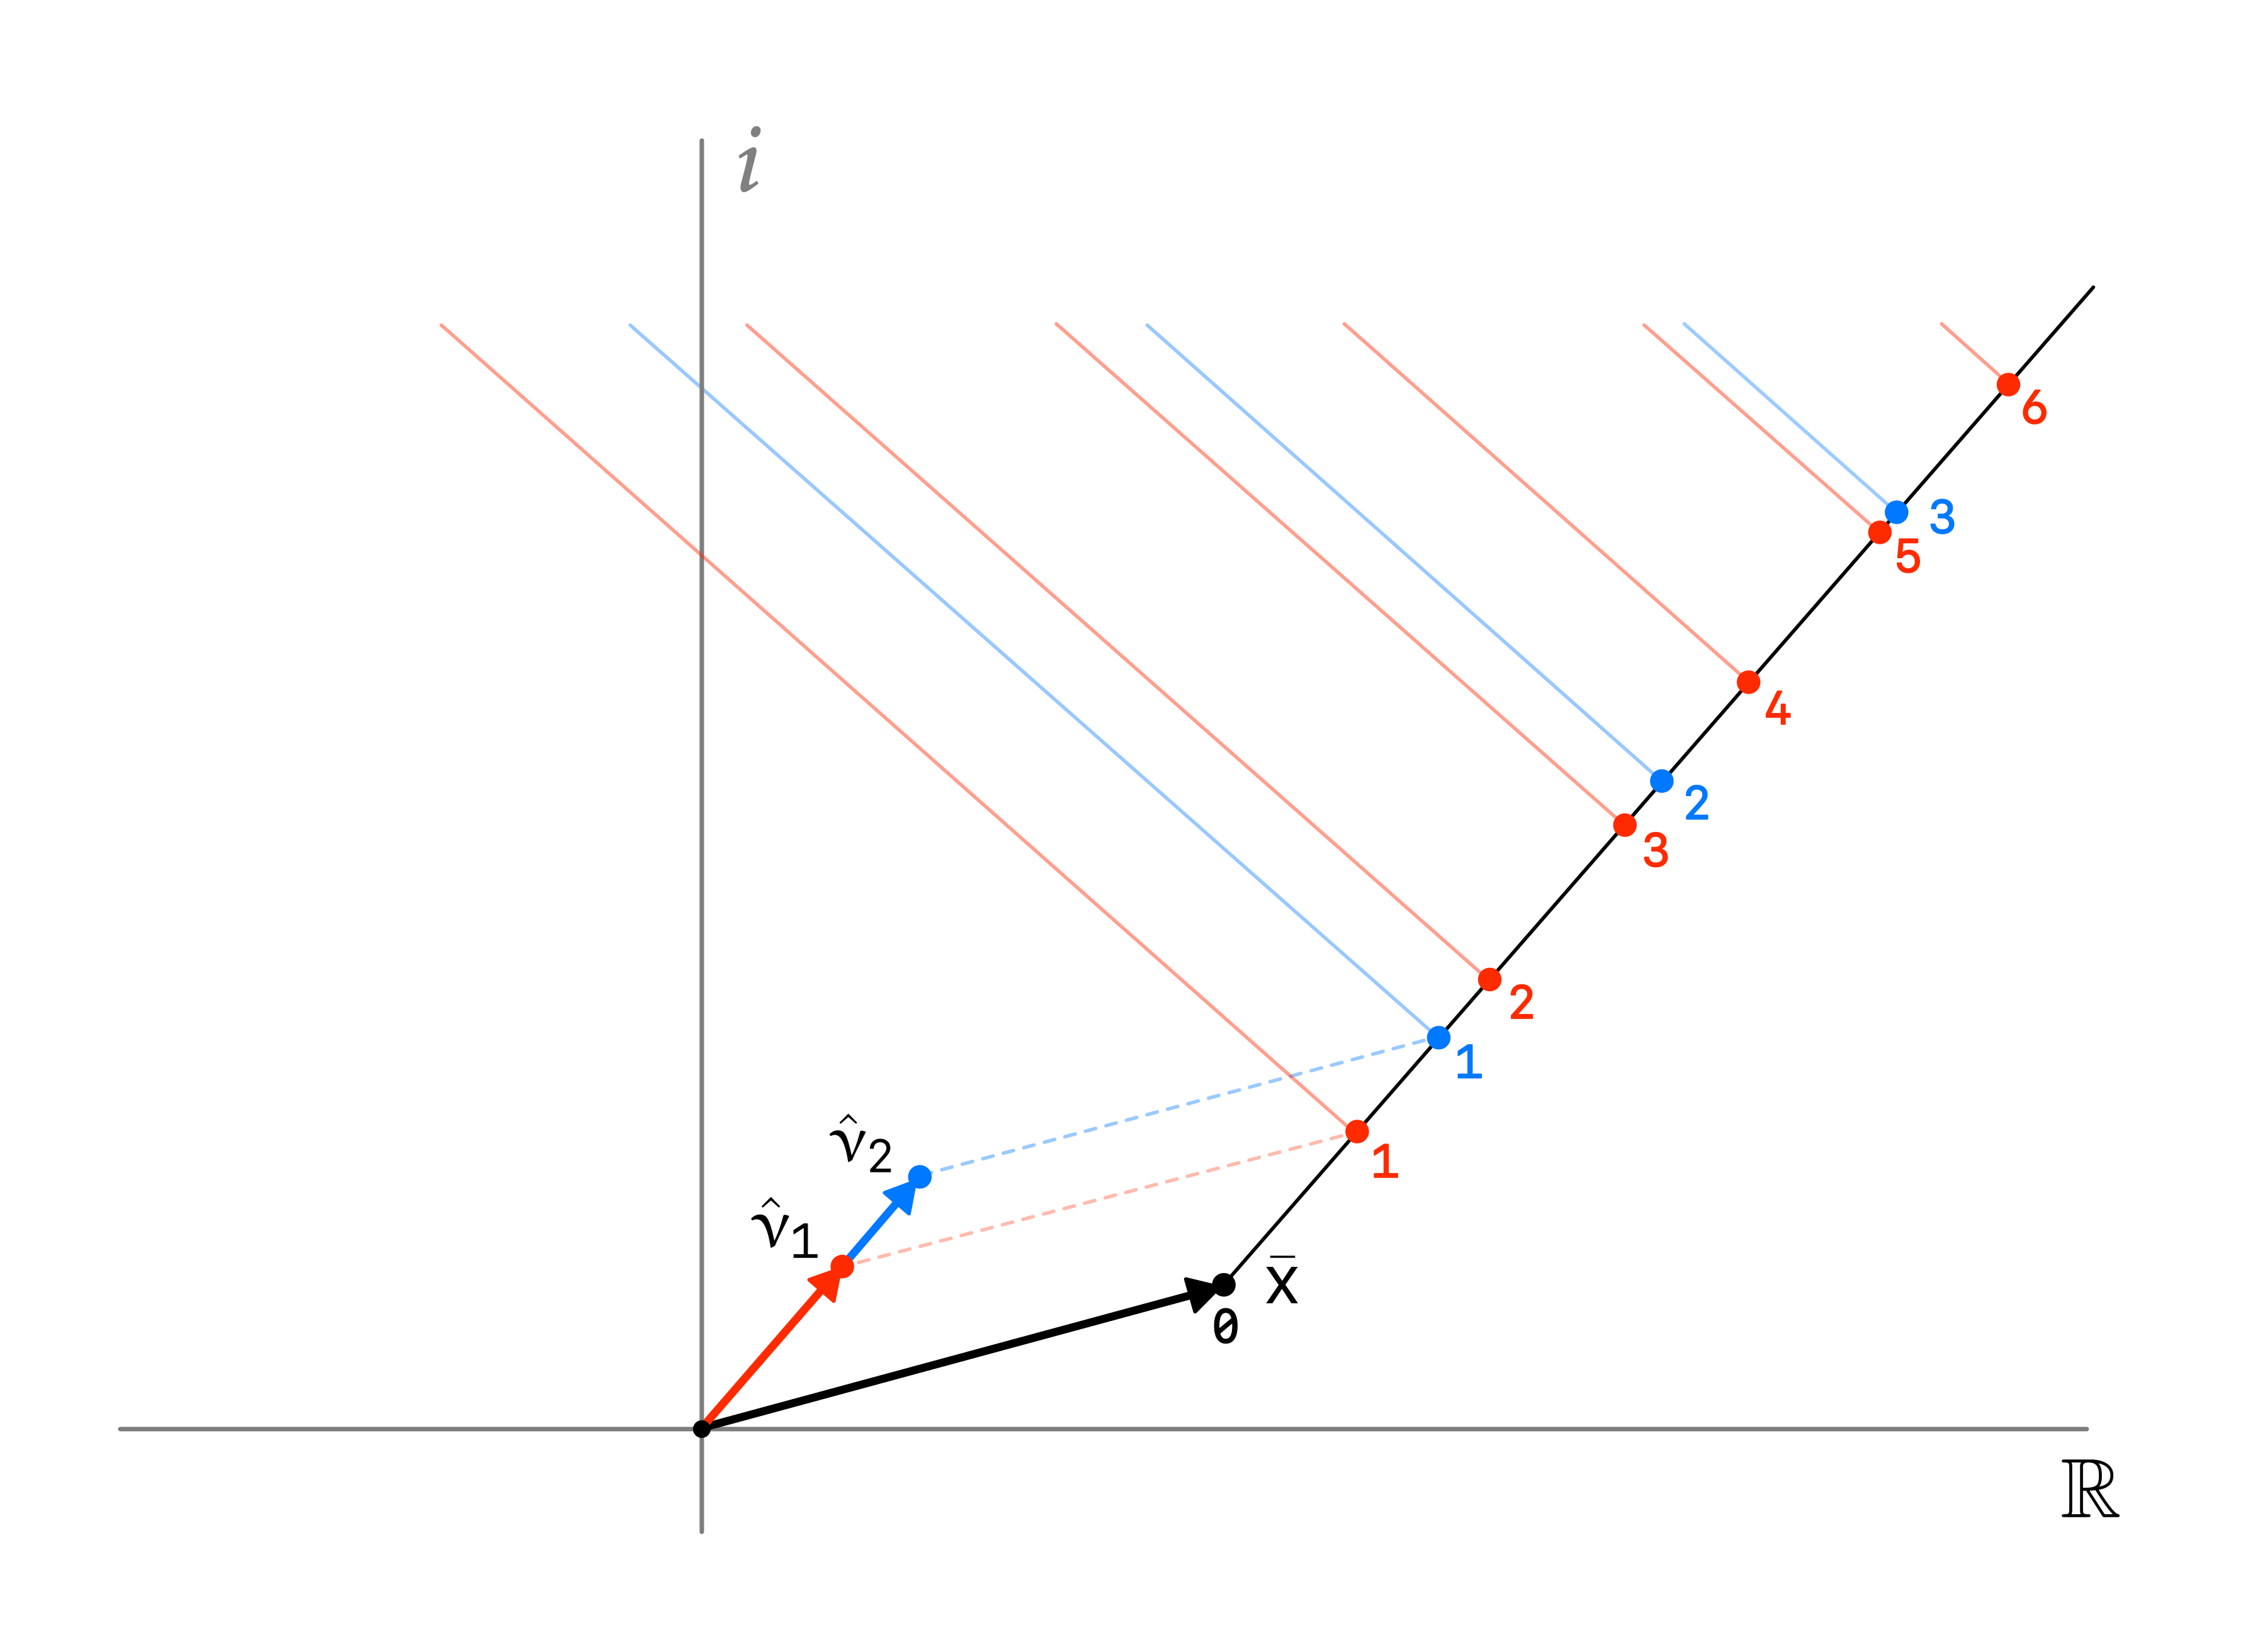
\includegraphics[width=75mm]{./img/complexMonoPeriods.png}\vspace{1mm}
    \captionof{figure}{\textls[-50]{\mono{Complex lattice generated by a mono-periodic function with linearly dependent complex periods}}}
    \label{fig:ci}
  \end{minipage}
  \noindent
  \begin{minipage}{\linewidth}
    \centering
    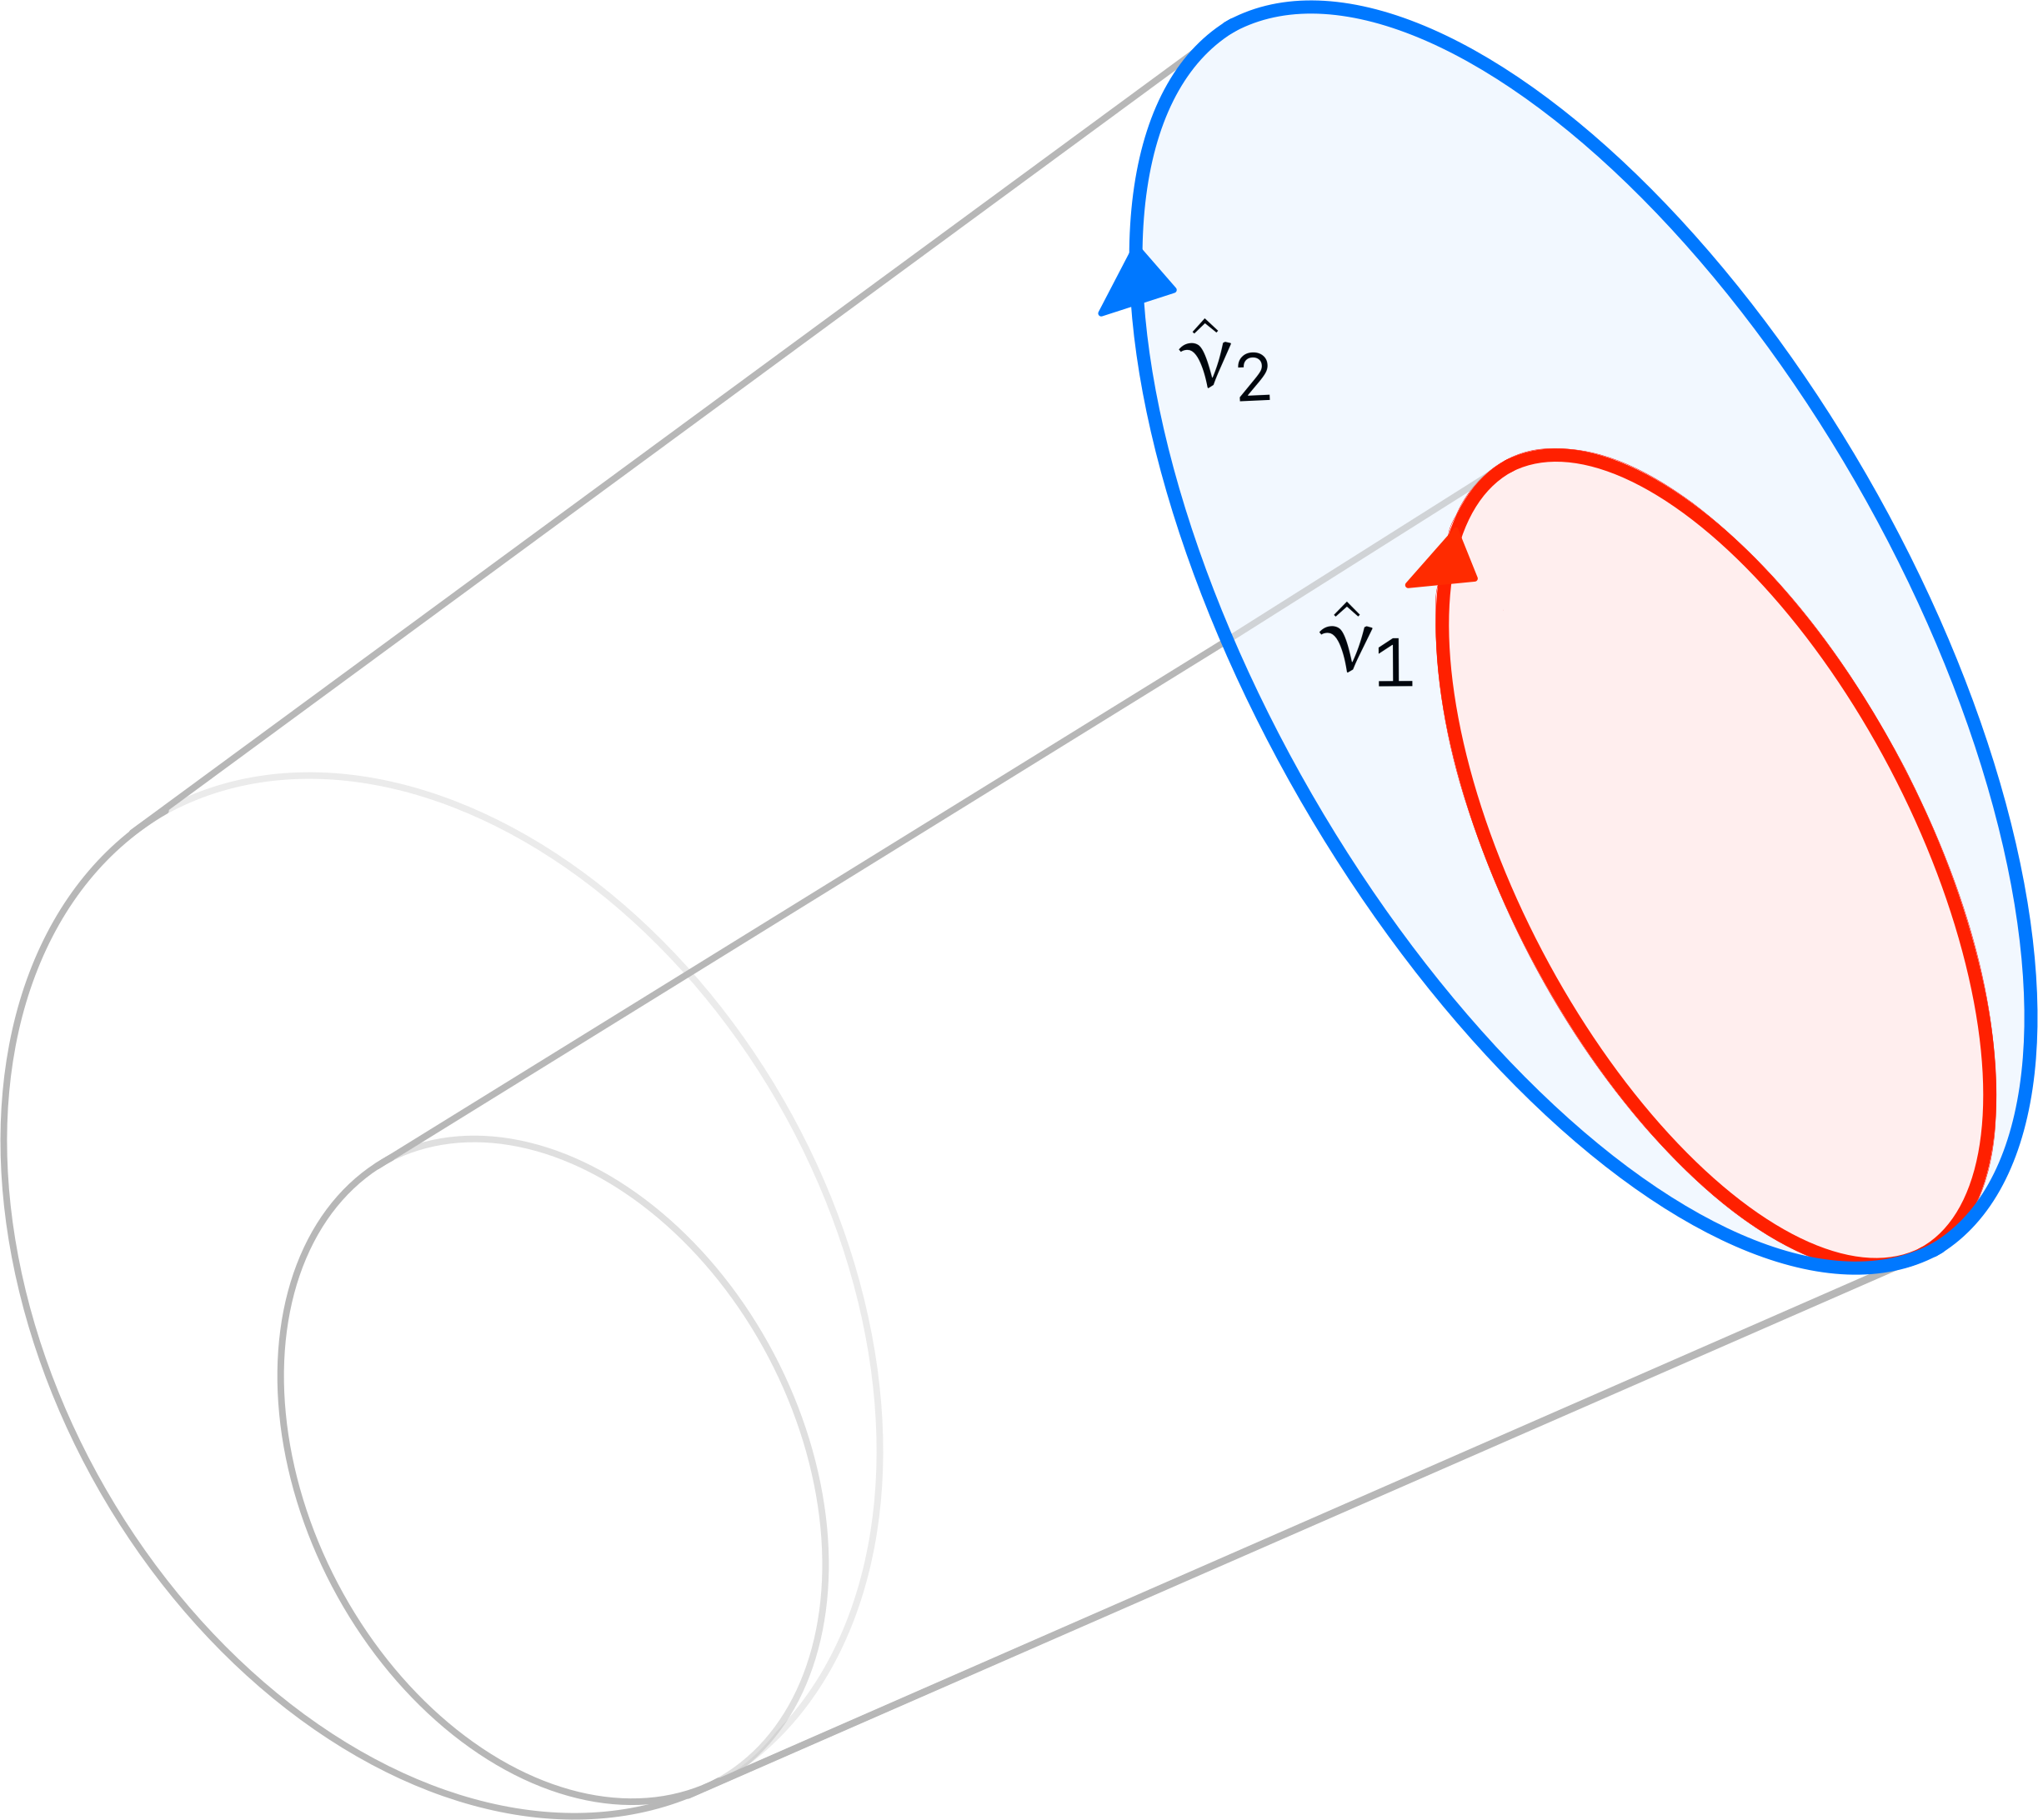
\includegraphics[width=59.1mm]{./img/complexCylinder.png}\vspace{1mm}
    \captionof{figure}{\textls[-50]{\mono{Cylindrical parameterisation of a complex lattice generated by a mono-periodic function}}}
    \label{fig:ec}
  \end{minipage}
\end{multicols}
\begin{flushleft}
  \textls[-50]{\mono{Fundamental theorems in vector algebra tell us that any two-dimensional vector space can have at most two independent basis vectors and any third vector can be written as a linear combination of those two bases. In the same way, any two-dimensional complex space is describable by at most two independent complex bases, in this case $\hat{\upomega}$\textsubscript{1} and $\hat{\upomega}$\textsubscript{2}. There cannot be third period $\hat{\upomega}$\textsubscript{3} since any such complex number will be reducible to $\hat{\upomega}$\textsubscript{3} = c\textsubscript{1}\,$\hat{\upomega}$\textsubscript{1} + c\textsubscript{2}\,$\hat{\upomega}$\textsubscript{2} with constants c\textsubscript{1},\,c\textsubscript{2}\;{$\in\;\mathbb{R}$}. It is possible for two complex periods to be linearly dependent though, in which case the generated lattice is effectively pseudo-bi-periodic and its parameterisation yields two coaxial complex cylinders; a example of this is shown in figures 5 and 6. When there is only one complex period, the generated lattice in that case is also strictly mono-periodic and forms a complex cylinder. This was the punchline of Jacobi's work: analytic functions can have either one complex period, or two (linearly) dependent complex bi-periods or two (linearly) independent complex bi-periods; among these three classes, only elliptic integrals appear to fall in the last category of independent bi-periods.\linebreak\linebreak
  }}
\end{flushleft}
\begin{flushleft}
  \textbf{\Large\pbold{REFERENCES}}\linebreak\linebreak
  \textls[-50]{\mono{
      [1] Intuitive Interpretation of Non-Interactive Zero-Knowledge Cryptography\linebreak
    }}
\end{flushleft}
\begin{flushright}
  \textbf{\large\pbold{METADATA}}\linebreak\linebreak
  \textls[-50]{\mono{
      \mono{Github: }\tcbox{}\linebreak
      \mono{Contracts: }\tcbox{}\linebreak
      \mono{Source: }\tcbox{}\linebreak
      \mono{SHA-1 Checksum: }\tcbox{}\linebreak
      \mono{Date: }\tcbox{\mono{\today}}\linebreak
    }}
\end{flushright}
\end{document}

%Note that the sine and cosine functions are defined by the coordinate transformation (x, y) = ({\large\pala\it{f}}\hspace{0.4mm}, {\large\pala\it{f}}\hspace{0.2mm}'\hspace{-1mm}) {\rightarrow} (sin{\,\uptheta}, cos{\,\uptheta}) which leads to a circle expressed in spherical coordinates.

